\documentclass[
  journal=medium,
  manuscript=Report,
  year=2023,
  volume=37,
]{cup-journal}

\usepackage{amsmath}
\usepackage[nopatch]{microtype}
\usepackage{booktabs}
\usepackage{comment}
\usepackage{subfigure}
\usepackage{indentfirst}
\setlength{\parindent}{2em}

\title{Wordle Game Reported Data Analysis}

\author{Yuxiao Yang}
\affiliation{Xi'an Jiaotong University, Xi'an, China}
\email[Yuxiao Yang]{sty0077777@gmail.com}

\keywords{Wordle; Correlation Analysis; SIR; GBDT; K-means; Word Difficult} %% First letter not capped

\begin{document}

\begin{abstract}
    In the year 2022, a word guessing game called Wordle has gained tremendous popularity on the internet. The purpose of this paper is to establish the relationship between word attributes and reported results, game modes and word difficulty, and to describe some interesting features of the data sets. We hope to bring insight and inspiration to the Puzzle Editor of the New York Times through the exploration and analysis of the data. Three models are established: Model I: Reported Number Prediction Model; Model II: GBDT Prediction Model; Model III: Word Difficulty Clustering Model. 
    
    For the former part of question 1, to explain the change in the number of reported results and predict the interval reported results in the future, we build the reported number prediction model: This model is optimized based on SIR Epidemic differential equation model combined with wordle real scenarios, and is solved iteratively in difference form. Key parameters in the model are obtained by single-objective optimization, and the model predicts that the number interval of reported results on March 1, 2013 will be (19381, 20383). The partial derivatives of the four parameters of the model are calculated and their slopes are observed. The slope of parameter $\alpha$ is the highest, indicating that it had the greatest influence on the model. Since there is no infinite value, the model performs well in sensitivity analysis. 
    
    For the latter part of question 1, to explore the correlation between word attributes and the percentage of hard mode, we extract the corresponding qualitative data and quantitative data of word attributes. Pearson Chi-square test and Spearman correlation coefficient are used respectively to find that there is no significant correlation between any word attributes and the percentage of hard mode. 

    For question 2, to predict the distribution of future report results for a given word, we build a GBDT Prediction Model. The model to extract the characteristics of 14, use the gradient promotion tree (GBDT) methods, respectively predicted seven tries percentage. We predict the 7 tries’ percentage of the ERRIE for [0.8, 9.3, 23.7, 30.31, 23,11.67, 2.74]. The uncertainty is mainly reflected in the low precision and small amount of data set, and the average absolute prediction error of the model is 2.36\%.

    For question 3, to classify words by difficulty, we build a word difficulty clustering Model: this model uses principal component analysis and K-means method to define difficulty by tries’ distribution. The clustering model introduces the model in problem 2, establishes the relationship between word attributes and difficulty, and calculates EERIE as medium difficulty. The analysis of word attributes shows that the difficulty of a word is inversely correlated with the word usage frequency and letters’ frequency, and positively correlated with the number of repeated letters and common combined letters. The accuracy of the model is 79\%. 

    For question 4, we made the correlation scatter diagrams of quantitative data in the data set, verified the positive correlation between tries and difficulty, also provided the research basis for the study of the correlation between the hard mode and the total number of reports. 

\end{abstract}

\section{Introduction}

\subsection{Problem Background}

In the year 2022, a word guessing game called Wordle has gained tremendous popularity on the internet. This game, offered by the New York Times, requires players to guess a five-letter word in six tries or less and provides feedback with every guess. The feedback is indicated by changing tile colors, where yellow indicates a correct letter in the wrong location, green indicates a correct letter in the correct location, and gray indicates an incorrect letter. Figure \ref{word} is an example solution of the correct result ‘cache’. One unique aspect of Wordle is that there is only one daily puzzle for all players worldwide, which adds a social element to the game when players share their results on social media platforms such as Twitter. Overall, Wordle is a simple but engaging game that has captivated players around the world. 

\begin{figure}[hbt!]
    \centering
    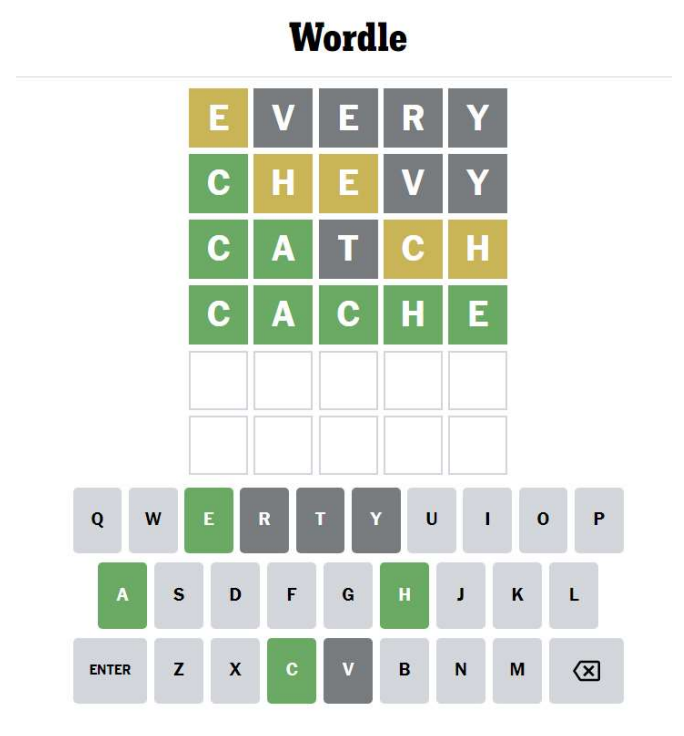
\includegraphics[width=0.6\linewidth]{pic/cache.png}
    \caption{Guessing the word ’cache’ }
    \label{word}
\end{figure}

\subsection{Research Questions}
    
1. The number of reported results vary daily. Develop a model to explain this variation and use your model to create a prediction interval for the number of reported results on March 1, 2023. Do any attributes of the word affect the percentage of scores reported that were played in Hard Mode? If so, how? If not, why not?

2. For a given future solution word on a future date, develop a model that allows you to predict the distribution of the reported results. In other words, to predict the associated percentages of (1, 2, 3, 4, 5, 6, X) for a future date. What uncertainties are associated with your model and predictions? Give a specific example of your prediction for the word EERIE on March 1, 2023. How confident are you in your model’s prediction?

3. Develop and summarize a model to classify solution words by difficulty. Identify the attributes of a given word that are associated with each classification. Using your model, how difficult is the word EERIE? Discuss the accuracy of your classification model.

4. List and describe some other interesting features of this data set.

\subsection{My Work}

The purpose of this subject is to establish the relationship between word attributes and reported results, game modes and word difficulty, and to describe some interesting features of the data sets. My work mainly includes the following:

\begin{enumerate}
    
\item 1. Establish the reported number prediction model, solve the model parameters according to the historical Data in the Data File, and use the model for prediction;

\item 2. Use Spearman correlation test and Pearson Chi-square test to analyze the correlation between word attributes and percentage of hard mode;

\item 3. Construct the report results distribution prediction model, predict ERRIE's tries distribution, and analyze the uncertainty and accuracy of the model;

\item 4. Define the classification of difficulty, establish the correlation between tries distribution and difficulty, and indirectly establish the relationship between word attributes and difficulty by introducing the prediction model of report result distribution, so as to construct the classification model of word difficulty. The difficulty of EERIE is evaluated by the model, and analyze the word characteristics and accuracy of the model under each classification;

\item 5. Exploratory analysis of other data in the Data File.

\end{enumerate}

In summary, the whole modeling process can be shown as follows (Figure \ref{work}):

\begin{figure}[hbt!]
    \centering
    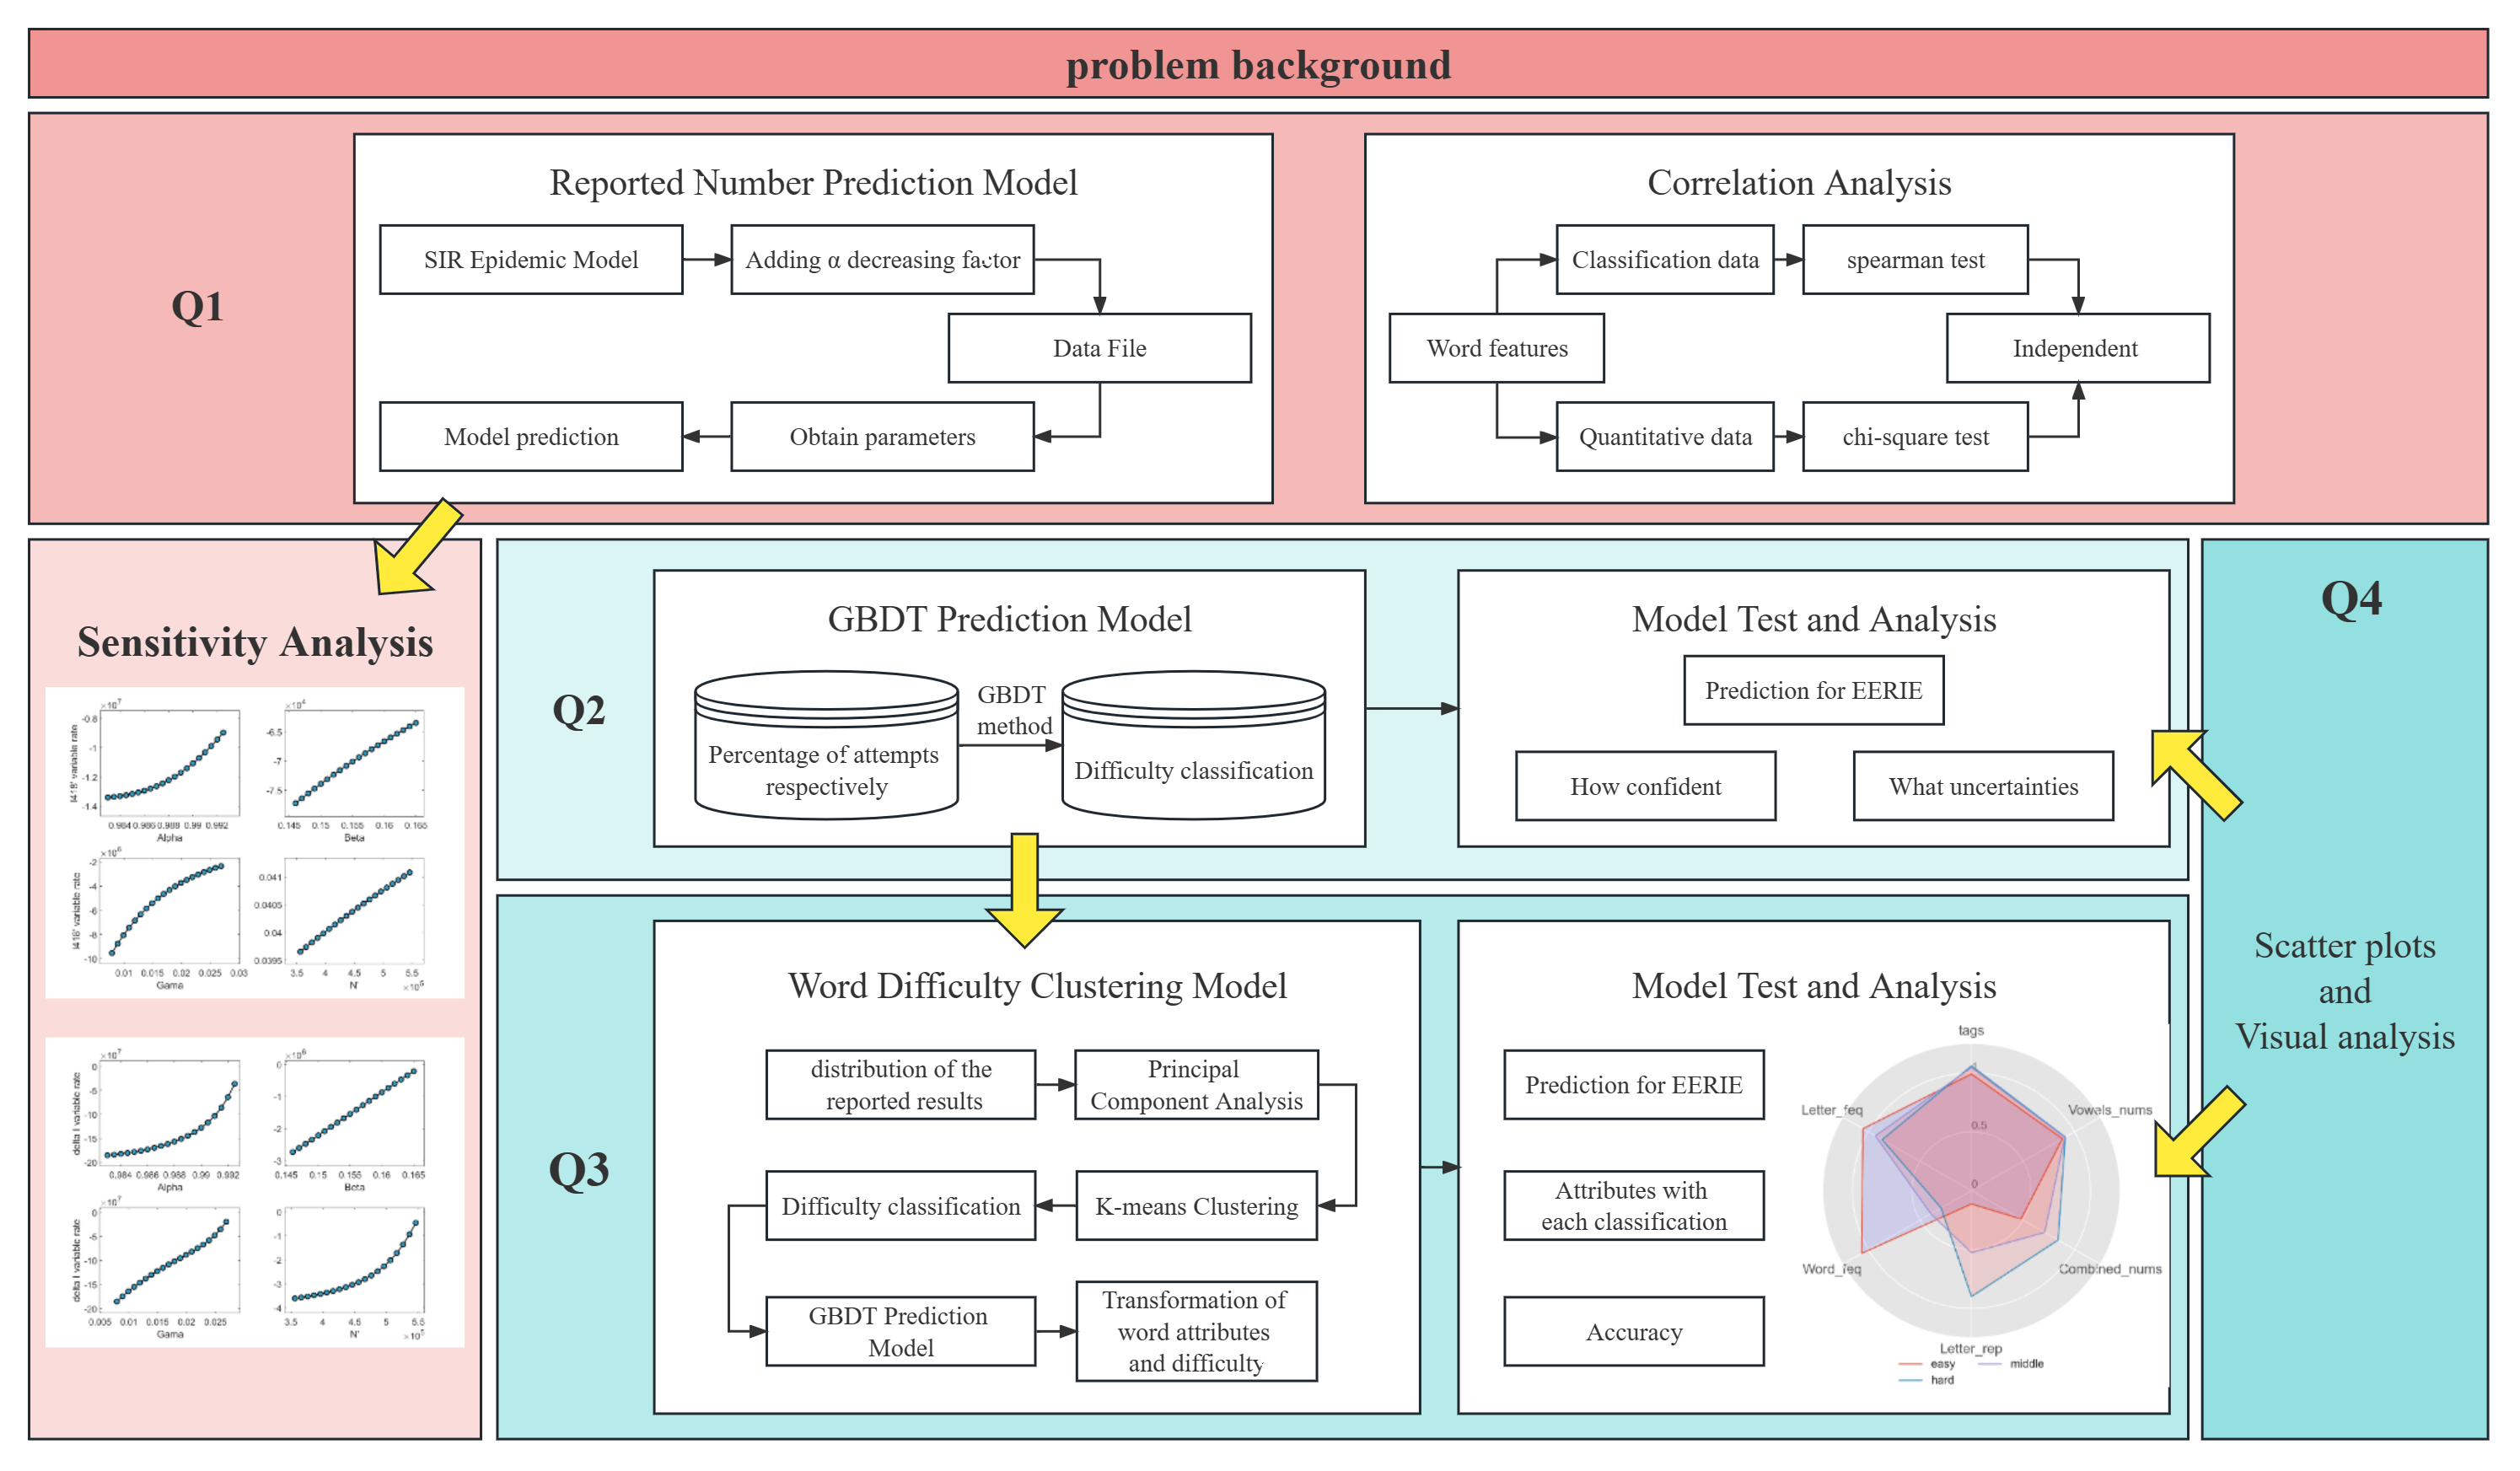
\includegraphics[width=\linewidth]{pic/our_work.png}
    \caption{My Work}
    \label{work}
\end{figure}

\subsection{Data Background Description}

MCM has generated a file of daily results for January 7, 2022 through December 31, 2022. This file includes the date, contest number, word of the day, the number of people reporting scores that day, the number of players on hard mode, and the percentage that guessed the word in one try, two tries, three tries, four tries, five tries, six tries, or could not solve the puzzle (indicated by X).

The data are described as follows (Table \ref{attribute}) :

\begin{table}[hbt!]
    \begin{threeparttable}
    \caption{Metadata}
    \label{attribute}
    \begin{tabular}{lll}
    \toprule
    \headrow Feature Name & Description & Type \\
    \midrule
    Date & The date in month-day-year format of a given Wordle puzzle. & datetime64 \\ 
    \midrule
    Contest number & An index of the Wordle puzzles, beginning with 202 on January 7, 2022. & int64 \\ 
    \midrule
    Word & The solution word players are trying to guess. & object \\ 
    \midrule
    Number of reported results & The total number scores that were recorded on Twitter that day. & int64 \\ 
    \midrule
    Number in hard mode  & The number of scores on Hard mode recorded on Twitter that day. & int64 \\ 
    \midrule
    1 try & The percentage of players solving the puzzle in one guess. & int64 \\ 
    \midrule
    2 tries & The percentage of players solving the puzzle in two guesses. & int64 \\ 
    \midrule
    3 tries & The percentage of players solving the puzzle in three guesses. & int64 \\ 
    \midrule
    4 tries & The percentage of players solving the puzzle in four guesses. & int64 \\ 
    \midrule
    5 tries & The percentage of players solving the puzzle in five guesses. & int64 \\ 
    \midrule
    6 tries & The percentage of players solving the puzzle in six guesses. & int64 \\ 
    \midrule
    7 or more tries (X) & The percentage of players that could not solve the puzzle in six tries. & int64 \\ 
    \bottomrule 
    \end{tabular}
    \end{threeparttable}
\end{table}

\section{Assumptions and Justifications}

To simplify the problem, we make the following basic assumptions, each of which is properly justified. 

$\bullet$ Assumption 1: The results reported is randomly sampled from all results at a constant proportion. 

Justification: The resulting data is based on the results shared on Twitter, but there are actually a lot more players. To simplify the analysis, we assume that the results reported is randomly sampled from all results at a constant proportion. 

$\bullet$ Assumption 2: As the number of days increases, the difficulty of the same words probably decreases. 

Justification: As the number of days increases, the user's proficiency increases, the words become easier to solve in fewer tries, and the difficulty of the same words probably decreases. Therefore, the number of date is an addition to the word, but is not considered an attribute of the word.

$\bullet$ Assumption 3: The solution word of wordle on March 1, 2023 is eerie. 

Justification: In question 2, on March 1, 2023, the word is EERIE. For the sake of problem 3, let's assume that this condition still holds.

\section{Notations}

The key mathematical notations used in this paper are listed in Table \ref{Notations}. 

\begin{table}[hbt!]
    \begin{threeparttable}
    \caption{Notations used in this paper}
    \label{Notations}
    \begin{tabular}{lll}
    \toprule
    \headrow Symbol & Description \\ 
    \midrule
    $S_n$ & The number who did not use wordle on date n\\ 
    \midrule
    $I_n$ & The number who used wordle on date n\\ 
    \midrule
    $R_n$ & The number who will no longer use wordle\\ 
    \midrule
    $R^2$ & The determination coefficient\\ 
    \midrule
    MAE & Mean absolute error\\ 
    \midrule
    SSE & The sum of the squared errors\\ 
    \midrule
    $C_k$ & The center class k\\ 
    \midrule
    $pc_i$ & The i principal component \\ 
    \bottomrule 
    \end{tabular}
    \end{threeparttable}
\end{table}

\section{Data Cleaning}

\subsection{Preliminary Data Exploration}

\begin{enumerate}
    \item Number of reported results and Number in hard mode (Figure \ref{combine}):
    
    \begin{figure}[!htbp]
        \centering
        \subfigure[Number of reported results]{
            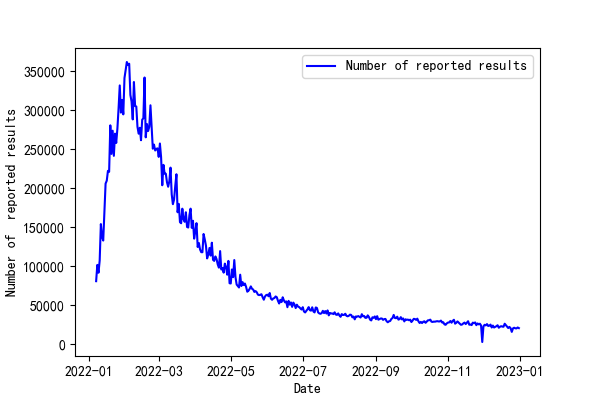
\includegraphics[width=0.49\linewidth]{pic/Number of reported results line plot.png}
            \label{Number of reported results}
        }
        \hfill
        \subfigure[Number in hard mode]{
            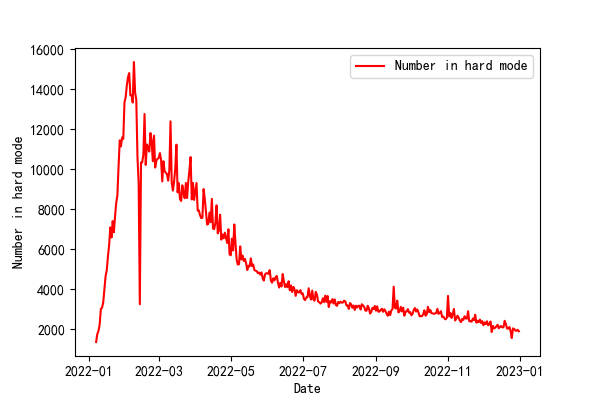
\includegraphics[width=0.49\linewidth]{pic/Number in hard mode line plot.png}
            \label{Number in hard mode}
        }
        \caption{Number of reported results plus hard mode}
        \label{combine}
    \end{figure}

    \item Word length characteristics:
    
    There are 355 words of length 5, 2 words of length 4, and 2 words of length 6.

\end{enumerate}

\subsection{Outlier Processing}

From the preliminary data exploration above, we found that there are three main issues with the dataset: 

1. There is a discontinuous mutation in the number of reports for certain days, which requires smoothing. 

2. The rule for wordle is 5 letter long words, but there are 4 letter long and 6 letter long cases.

3. The sum of trials does not accumulate to 100\%.

Therefore, we cleaned the dataset as follows:

1. Smoothing the abnormal points and taking the average value of the two days before and after to replace the original Outlier.

2. For words with abnormal length, we search for the closest word to fill in.

3. Normalize the tries so that the sum of the results is equal to 100.

\section{Model I: Reported Number Prediction Model and Correlation Analysis}

With the increase of the number of days, the reports participants present a regular change. This change is determined by its internal dynamic’s principle. Introducing the iterative solution of infectious disease model can maximize the mining of data information. 

Two types of attributes should be considered for the effect of word attributes on the percentage of hard mode. One is the categorical attribute and the other is the quantitative attribute. By calculating the relationship between these two attributes and the percentage separately, you can analyze whether the percentage is affected by them. 

\subsection{SIR Epidemic Differential Model}

According to assumption 1, the results reported is randomly sampled from all results at a constant proportion. Based on the potential number of wordle $N$ , we assume that the person who did not use wordle on day $n$ as $S_n$ , the person who used as $I_n$ and $I_n'$ participate in the report, while the true case of the participation is $I_n''$ . The person who will no longer use wordle as $R_n$. Therefore, for the target groups, an epidemic model is established to describe the number of users varies daily, which can be expressed as formula below and Figure \ref{SIR}.

\[
\begin{cases}
    I_{n+1} - I_{n} = \beta I_n \frac{S_n}{N}-\gamma_n I_n \\
    R_{n+1} - R_{n} = \gamma_n I_n  \\
    \gamma_n = \gamma_{n+1}\alpha  \\
    S_{n+1}-S_{n} = -\beta I_n \frac{S_n}{N}\\
    S_n + I_n + R_n = N \\
\end{cases}
\]

\begin{figure}[hbt!]
    \centering
    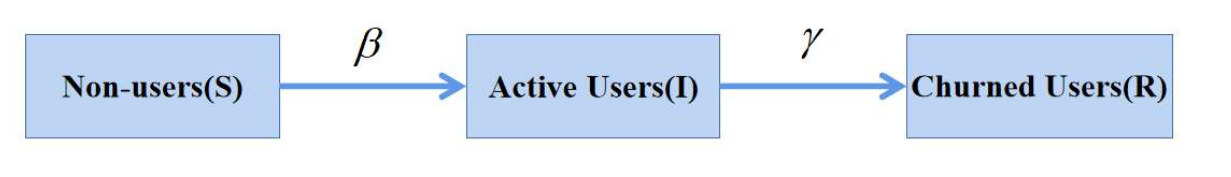
\includegraphics[width=0.7\linewidth]{pic/SIR.png}
    \caption{epidemic model}
    \label{SIR}
\end{figure}

here $\gamma_n$ is the proportion of $I_n$ converted to $R_n$ on the date n, $\alpha$ is the attenuation coefficient of $\gamma_n$ , and $\beta$ is the proportion of $S_n$ converted to $I_n$. In order to find the optimal parameter, we need to minimize the value of the following formula.

$$s.t. \quad min \sqrt{\sum_{n=1}^{357}(I_n'-I_n'')^2} = \Delta \overline{I}$$

From January 7, 2022 to March 1, 2023, experience 418 days. And for the data set, from January 7, 2022 to December 31, 2022, experience 359 days. We missed two words altogether. Therefore, the prediction interval is ($I_{418}' - \frac{\Delta \overline{I}}{357},I_{418}' + \frac{\Delta \overline{I}}{357}$)

\subsection{Feature Extraction}

In order to determine if word characteristics influence the proportion of hard mode, it is necessary to extract several features of words. This study extracted various word features such as the frequency of letters, frequency of word usage, count of repeated letters, presence of common combined letters, parts of speech, and number of vowels. These features were considered as potential factors that may impact the percentage of hard mode. Here is a detailed explanation of these features. 

\subsubsection{Qualitative Data}

$\bullet$ Part of speech: A part of speech is a category assigned to a word based on its syntactic and semantic properties. 

\subsubsection{Quantitative data}

$\bullet$ Frequency of letters: Extract all the words in Oxford Dictionary and classify the same letters to get the letter frequency characteristics of the words. 

$\bullet$ Frequency of word usage: Literature data from 2000 to present were extracted to obtain the usage frequency of the specified words. 

$\bullet$ Number of repeated letters: Number of repeating letters in a specified word. 

$\bullet$ Common combined letters: Especially al, ic, er, or at the end of words. 

$\bullet$ Number of vowels: Since vowels are an easily recognized feature in words, we counted the number of A, E,I, O, U to represent the number of vowels. 

\subsection{Correlation Analysis}

\subsubsection{Pearson Chi-Square Test}

First of all, we use Natural Language Toolkit dataset in python to classify the parts of speech of these words, which is nonquantitative variable. Then, the relationship between the parts of speech and the percentage of hard mode is inferred by using the hypothesis testing method. 

The qualitative data is suitable for frequency statistics, so Pearson Chi-square test is selected in this paper to analyze sample data. The percentage of hard mode and word part of speech were taken as two variables, and the difference between the two variables was demonstrated by Chi-square test. 

The statistical formula of chi-square test is shown in the formula below: 

$$\chi^2 = \sum \frac{(A-E)^2}{E} = \sum^m_{i=1}\sum^n_{j=1}\frac{(A_{ij}-Np_{ij})^2}{Np_{ij}}$$

In the formula, $N$ is the total number of words after data processing, $i$ is the partition variable hard mode percentage and $j$ is the partition variable for the part of speech. $A_{ij}$ represents the actual value of the frequency of the $i$ , $j$ values respectively, and $p_{ij}$ represents the expected probability of the frequency of the $i$ , $j$ values respectively. Take the median of the percentage of hard mode and divide it according to it. If it is lower than the median, it is called less, and if it is higher than the median, it is called more. 

In this Chi-square test model, we set the Null hypothesis: observed frequency of variable does not differ from expected frequency under independent condition; alternative hypothesis: observed frequency of variable does not differ from expected frequency. If adjoint probability P>0.05, then the null hypothesis is accepted and the variables are independent of each other. 

\subsubsection{Spearman Correlation Coefficient}

The quantitative data is suitable for variable relationship analysis, so Spearman correlation coefficient is selected in this paper to analyze sample data. The percentage of hard mode and each word features were taken as two variables, and the correlation coefficient between the two variables was demonstrated by Spearman test. At the same time, the relationship between variables at the significance level was also tested The statistical formula of Spearman correlation coefficient is shown in the formula below.

$$\rho_s = \frac{\sum^N_{i=1}(R_i - \overline{R})(S_i - \overline{S})}{[\sum^N_{i=1}(R_i - \overline{R})^2\sum^N_{i=1}(S_i - \overline{S})^2]^{\frac{1}{2}}}$$

Where $N$ is the total number of words after data processing, $R_i$ and $S_i$ are the values of variates, $\overline{R}$ and $\overline{S}$ are averages. 

\subsection{Results}
\subsubsection{SIR Epidemic Model}
\begin{enumerate}
    \item Parameter Estimation
    
    By traversing search the formula from large scale to small scale and iterating according to the number of days, we get the value of each parameter. The potential number of reports $N' = 578000$ , the proportion of $S_n$ converted to $I_n$, $\beta = 0.1645$, the attenuation coefficient of $\gamma_n, \alpha = 0.9925$ and $\gamma_0 = 0.0300$.
    \item Calculation Results 
    
    According to the above parameters, we get $min \sqrt{\sum_{n=1}^{357}(I_n'-I_n'')^2} = \Delta \overline{I} = 1.9807 \times 10^5$,$I_{418}' = 19882$. Therefore, the prediction interval is (19381, 20383). 
    
    We plot the central value $I_n'$ against date $n$ and get the figure \ref{SIR real} below. 
    
    \begin{figure}[hbt!]
        \centering
        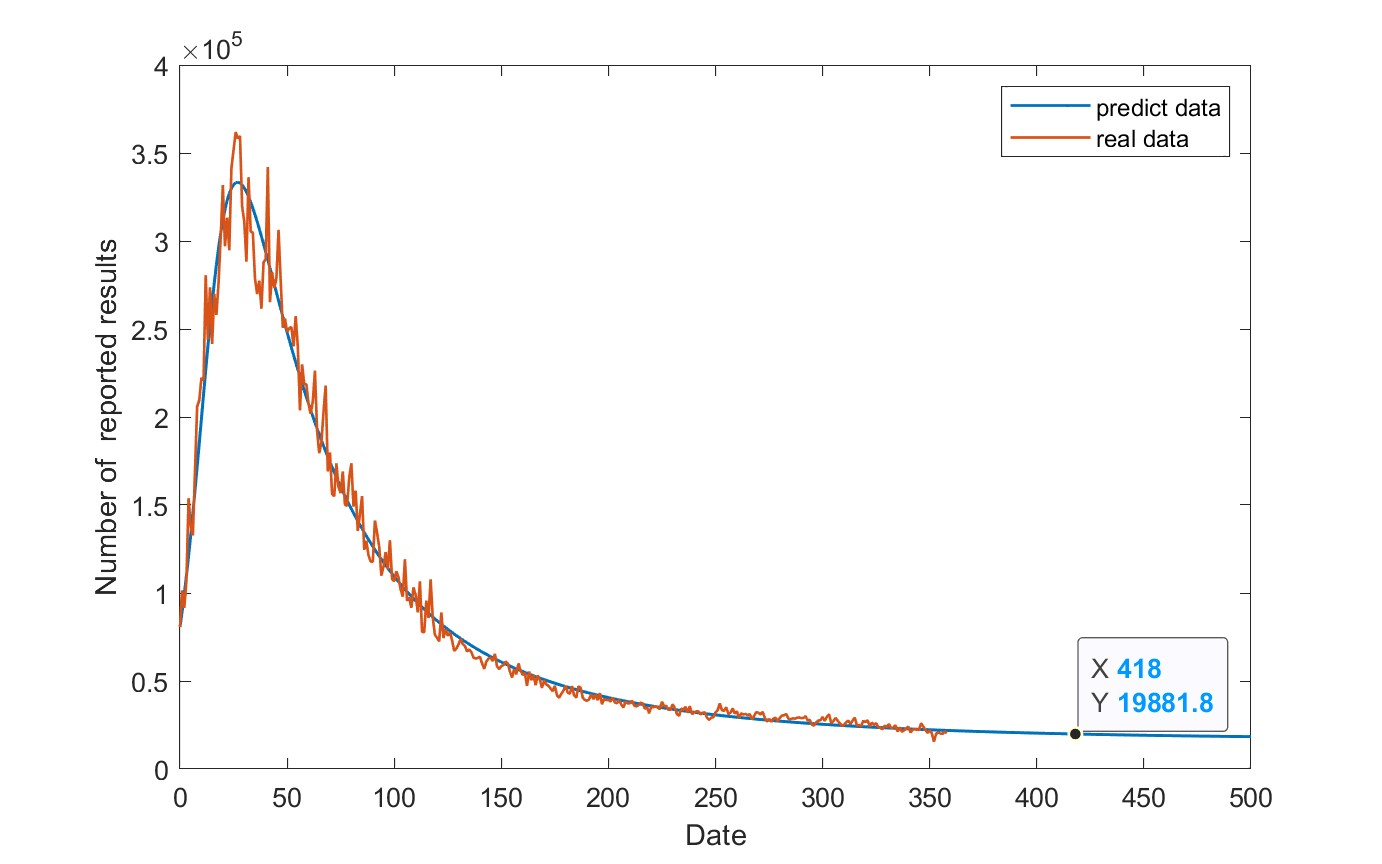
\includegraphics[width=0.7\linewidth]{pic/SIR_real.jpg}
        \caption{SIR epidemic model prediction}
        \label{SIR real}
    \end{figure}

    From the figure \ref{SIR real}, we can see that in the previous forecast, the general trend of the real data is similar to the forecast data, that is, the number of people participating in the report has increased rapidly since the data start time January 7, 2022. It reached a maximum at date 35-30, and then began to decline rapidly, leveling off after about 100 days. At around date 350, the decline is very slow, so there should be little difference between the desired $I_{418}'$ and the final value of December 31, 2022, and the calculated result is consistent. 
\end{enumerate}

\subsubsection{Feature extraction}
\begin{enumerate}
    \item  Quantitative data 
    
    We use Natural Language Toolkit dataset in python and find that adjective and noun are the main parts of speech. If the percentage of hard mode is lower than the median, it is called less, and if it is higher than the median, it is called more. Therefore, the selection method of variables $i$ , $j$ are shown in table \ref{variables}.

    \begin{table}[hbt!]
        \begin{threeparttable}
        \caption{The selection method of variables}
        \label{variables}
        \begin{tabular}{llll}
        \toprule
        \headrow Variate & 0 & 1 & 2 \\ 
        \midrule
        $i$ & Less & More & /\\ 
        \midrule
        $j$ & adj & N & others\\ 
        \bottomrule 
        \end{tabular}
        \end{threeparttable}
    \end{table}

    In this question, the conclusion of the chi square test of hard mode percentage and part of speech variables is in table \ref{square test result}: 

    \begin{table}[hbt!]
        \begin{threeparttable}
        \caption{square test result}
        \label{square test result}
        \begin{tabular}{llllllll}
        \toprule
        \headrow Content & Category & Adj. & N. & others & total & $\chi^2$ & P \\ 
        \midrule
        hard mode percent & Less & 3 & 59 & 4 & 66 &  & \\ 
        \midrule
        hard mode percent & More & 14 & 260 & 19 & 293 & 0.024 & 0.988\\ 
        \midrule
        total &  & 17 & 319 & 23 & 359 &  & \\ 
        \bottomrule 
        \end{tabular}
        \end{threeparttable}
    \end{table}

    Because adjoint probability $P \geq 0.05$, then the null hypothesis is accepted and the variables are independent of each other. Therefore, parts of speech of the words don’t affect the Hard Mode percentage of scores reported. 

    \item  Qualitative Data
    \begin{table}[hbt!]
        \begin{threeparttable}
        \caption{Correlation coefficients results}
        \label{Correlation coefficients results}
        \begin{tabular}{lllllll}
        \toprule
        \headrow & Hard Percent & Vowels nums & Combined nums & Letter freq & Letter rep & Word freq\\ 
        \midrule
        hard percent  & 1 & 0.09 & 0.055 & -0.049 & 0.082 & 0.105 \\ 
        \bottomrule 
        \end{tabular}
        \end{threeparttable}
    \end{table}

    According to the table \ref{Correlation coefficients results}, we can find that all the correlation coefficients are less than 0.15, which proves that the correlation between variables is small, that is, the hard mode percentage has nothing to do with the word attribute.
\end{enumerate}

\section{Model II: GBDT Prediction Model}

In order to predict the distribution of future report results for a given word, we conducted report result distribution prediction. We extracted the features of the words, used the GBDT method to predict seven tries percentages respectively, obtained the predicted value of ERRIE's tries percentage, and carried out uncertainty analysis according to the algorithm.

\subsection{GBDT Prediction Algorithm}

Based on the question 1, we extract the word features and attach the attributes of time and letter arrangement. Take the five letters that make up the word, and count them as five features. The number of months, weeks and days are taken as three features, and the six features in the question 1 are added to make a total of 14 word features. 

In order to get the prediction result, we introduce the GBDT prediction model. The core idea of GBDT is weighted residual error fitting, that is, in each round of training, the model will calculate the sample residual error according to the results of the previous round of training, and take the residual error as a new target variable for training. At the same time, in order to prevent overfitting, the model will also prune and limit the depth of each decision tree. Its core algorithm is shown below.

The original data was randomly divided into training set and test set, in which training set accounted for 80\% and test set accounted for 20\%. The GBDT algorithm is trained with the training set. The algorithm solves the relationship between a word and the percentage of tries. The parameters are adjusted to minimize the sum of the average absolute errors of the seven tries of the test set, and the optimal parameters are obtained. Since the percentages of tries are predicted separately, the sum of the seven percentages often does not add up to 100\%.

\begin{figure}[hbt!]
    \centering
    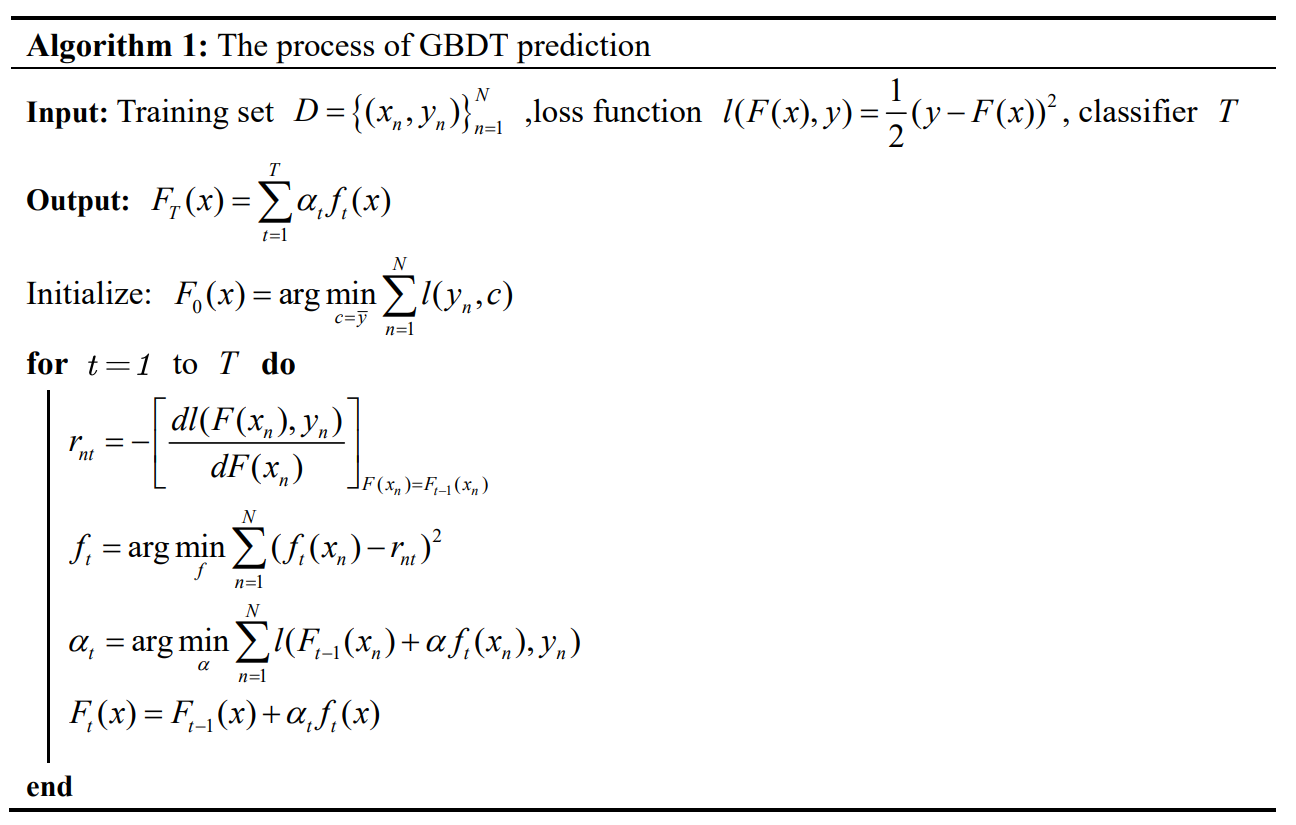
\includegraphics[width=0.9\linewidth]{pic/GBDT伪代码.png}
    \label{GBDT}
\end{figure}

\subsection{Results}
\subsubsection{Prameters Setting}

For the seven predicted targets ('1 try', '2 tries', '3 tries', '4 tries', '5 tries', '6 tries', '7 or more tries (X)'), we used the gradient boosting decision tree (GBDT) machine learning method for prediction. Using the GridSearchCV method, we selected certain important attributes to train the GBDT and obtained the optimal parameters. The optimal parameters are explained as follows: 

Learning rate: The learning rate determines whether and when the objective function can converge to a local minimum. 

n estimators: This parameter specifies the number of weak classifiers. Larger value might lead to better accuracy. 

max depth: This parameter is related to pruning. The larger the max depth, the more information about the data can be captured. 

min samples leaf: This parameter specifies the minimum samples required to be at a leaf node. 

For the 7-prediction model, the best parameters and corresponding fitting effects are shown in the table \ref{best parameters} below: 

\begin{table}[hbt!]
    \begin{threeparttable}
    \caption{The best parameters and corresponding fitting effects}
    \label{best parameters}
    \begin{tabular}{lllll}
    \toprule
    \headrow Object & learning rate & n estimators & max depth & min samples leaf\\ 
    \midrule
    1 try & 0.1 & 50 & 5 & 1 \\ 
    \midrule
    2 tries & 0.1 & 100 & 2 & 5 \\ 
    \midrule
    3 tries & 0.1 & 100 & 3 & 5 \\ 
    \midrule
    4 tries & 0.1 & 100 & 2 & 1 \\ 
    \midrule
    5 tries & 0.1 & 100 & 2 & 1 \\ 
    \midrule
    6 tries & 0.1 & 100 & 3 & 5 \\ 
    \midrule
    7 tries & 0.1 & 100 & 2 & 5 \\ 
    \bottomrule 
    \end{tabular}
    \end{threeparttable}
\end{table}

\subsubsection{Results Evaluation}

    For each of the prediction result, we use $R^2$ and MAE (Mean Absolute Error) as evaluating indicators. 

$$MAE(y,\widehat{y}) = \frac{1}{m}\sum_{i=1}^{m}(|y_i - f(x_i)|)$$

Where $y_i$ is the true value and $f(x_i)$, $\widehat{y}$ are the predicted value of the model. $R^2$ is the determination coefficient, which is used to measure the proportion of the variability in the dependent variable that can be explained by the independent variable. The closer $R^2$ is to 1, the better the model’s performance. 

\begin{table}[hbt!]
    \begin{threeparttable}
    \caption{The value of $R^2$ and MAE}
    \label{MAE}
    \begin{tabular}{lllll}
    \toprule
    \headrow Evaluation index & $R^2$(train)  & $R^2(test)$ & MAE(train) & MAE(test)\\ 
    \midrule
    1 try & 0.98 & 0.79 & 0.07 & 0.09 \\ 
    \midrule
    2 tries & 0.78 & 0.59 & 1.27 & 1.68 \\ 
    \midrule
    3 tries & 0.87 & 0.68 & 2.14 & 2.84 \\ 
    \midrule
    4 tries & 0.60 & 0.41 & 2.75 & 3.33 \\ 
    \midrule
    5 tries & 0.74 & 0.51 & 2.40 & 3.89 \\ 
    \midrule
    6 tries & 0.87 & 0.52 & 1.75 & 2.83 \\ 
    \midrule
    7 tries & 0.49 & 0.57 & 1.96 & 1.85 \\ 
    \midrule
    Mean & 0.76 & 0.58 & 1.76 & 2.36 \\ 
    \bottomrule 
    \end{tabular}
    \end{threeparttable}
\end{table}

The prediction result is good. Performance of each model on test set is: the average $R^2$ is 0.58, MAE is 2.36, indicating that the result is accurate.

One single model ‘3 tries’ is selected for specific analysis, whose performance is relatively better, in order to analyze which feature has the most significant influences on the probability. First, here is the visualization of contrast between prediction values and true values in both training set and test set.

\begin{figure}[!htbp]
    \centering
    \subfigure[Train set]{
        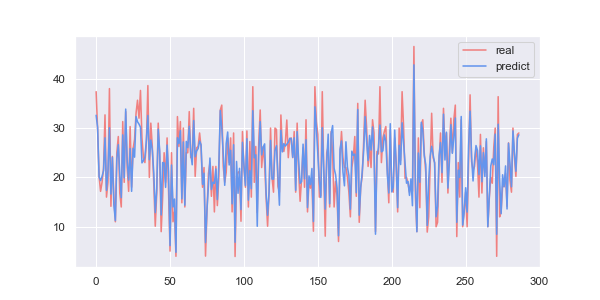
\includegraphics[width=0.49\linewidth]{pic/3 tries训练图.png}
        \label{Train set}
    }
    \hfill
    \subfigure[Test set]{
        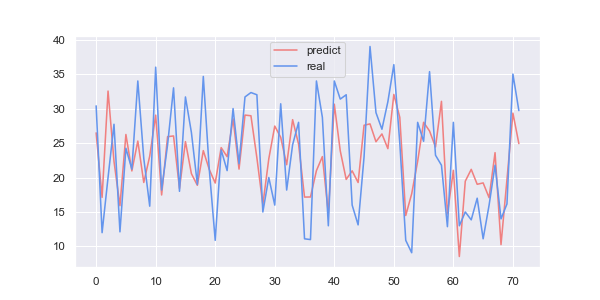
\includegraphics[width=0.49\linewidth]{pic/3 tries测试图.png}
        \label{Test set}
    }
    \caption{Contrast between prediction values and true values in data set}
    \label{combine2}
\end{figure}  

\subsubsection{Figure Explanation}

SHAP package could enable us to visualize the process of machine learning. SHAP has two cores, namely SHAP values and SHAP interaction values.

SHAP model explains the model's prediction as the sum of the attribution values of each input feature, where the attribution value is the SHAP value. According to the formula below.

$$y' = \phi_0 + \sum_{i=1}^{M}\phi_i$$

Where every feature has a corresponding SHAP value, which is also called $\phi_i$. And $\phi_0$ is the constant for interpolating the model, which is actually the mean prediction of all training samples.

\begin{figure}[!htbp]
    \centering
    \subfigure[The global importance of the feature]{
        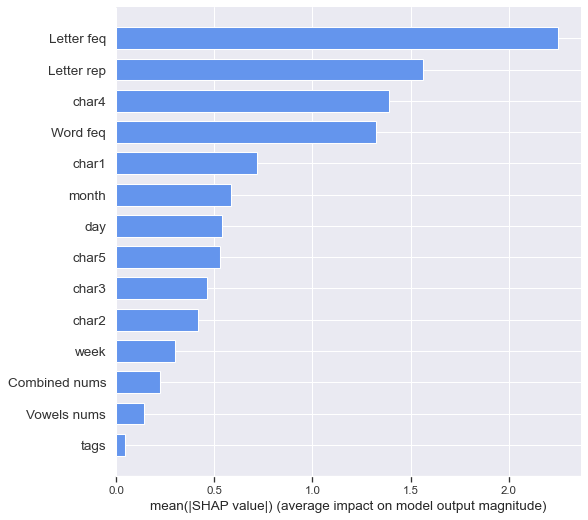
\includegraphics[width=0.49\linewidth]{pic/feature importance.png}
        \label{The global importance of the feature}
    }
    \hfill
    \subfigure[Distribution of characteristic values]{
        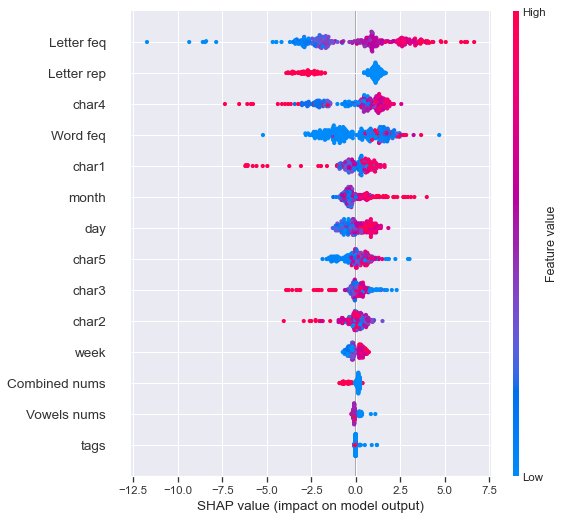
\includegraphics[width=0.49\linewidth]{pic/feature value.png}
        \label{Distribution of characteristic values}
    }
    \caption{Feature importance and values}
    \label{combine3}
\end{figure}

The average absolute value of SHAP values of each feature is taken to obtain the standard bar diagram, whose value represents the global importance of the feature. At the same time, we can also simply draw SHAP values of each feature of each sample through scatter points, and the relationship between the size of characteristic values and the predicted impact can be seen through color, as well as the distribution of its characteristic values.

It can be found that in case of 3 tries, the first four characteristics, namely the frequency of letters, the number of repeated letters, the letter in the fourth position, and the frequency of word use contribute the most to the accuracy of prediction.

\subsubsection{Uncertainty}

(1) There is a rounding process from the actual percentage to the reported percentage, which makes the training data generally appear errors and reduces the training effect;

(2) Due to the small amount of data, the accuracy of prediction using machine learning algorithm may not be high enough;

(3) It may be that key features are not all extracted and used for training.

\subsubsection{‘Eerie’ Prediction}

For the word EERIE, we predict that its percentage on each try is respectively shown in the table \ref{prediction}.

\begin{table}[hbt!]
    \begin{threeparttable}
    \caption{The contribution of each feature prediction}
    \label{prediction}
    \begin{tabular}{lllllll}
    \toprule
    \headrow 1 try & 2 tries & 3 tries & 4 tries & 5 tries & 6 tries & 7 tries\\ 
    \midrule
    0.8 & 9.32 & 23.74 & 30.31 & 23.02 & 11.66 & 2.74\\ 
    \bottomrule 
    \end{tabular}
    \end{threeparttable}
\end{table}

\begin{figure}[hbt!]
    \centering
    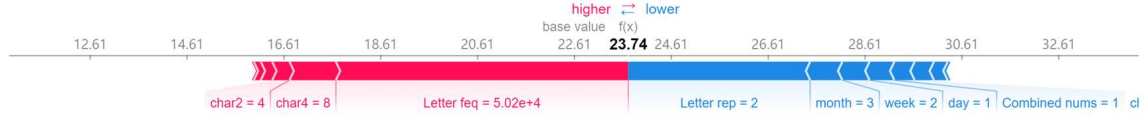
\includegraphics[width=\linewidth]{pic/单词特征影响.jpg}
    \caption{The contribution of each feature prediction}
    \label{feature influence}
\end{figure}

Meanwhile, we can analyze the contribution of each feature prediction result by using the model used in 3 tries. For the red one, it is positive contribution, while for the blue one, it is negative contribution. It can be interpreted from the figure \ref{feature influence} above that the positive contribution of the feature Letter feq $=$ 50000 is the largest, followed by char4 $=$ 8. But the negative contribution of Letter rep $=$ 2 is large, followed by month $=$ 3. Under the combined influence of all features, the predicted value of 3 tries percentage of EERIE in this sample is 23.74.

\subsubsection{Model Verification}

\begin{figure}[hbt!]
    \centering
    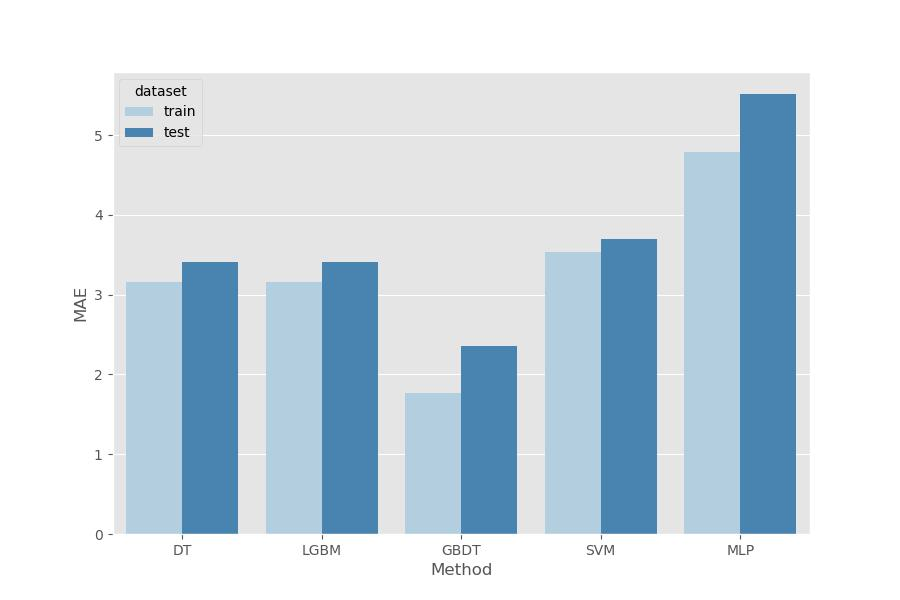
\includegraphics[width=0.6\linewidth]{pic/各方法对比图.jpg}
    \caption{The effectiveness of model}
    \label{effectiveness}
\end{figure}

Finally, in order to verify the effectiveness of our model, we selected other four models to compare their training error MAE, which are Decision Tree Regressor, LGBM, SVM, MLP Regressor. The results (Figure \ref{effectiveness}) show that our model has better performance.

\section{Model III: Word Difficulty Clustering Model}

The question focuses on how to establish a relationship between word features and difficulty. As the number of tries required to solve a word is inherently linked to its difficulty, and the model II is used to determine the relationship between word features and the number of tries. By utilizing the number of tries as a connecting bridge, an indirect correlation can be drawn between word features and difficulty, ultimately leading to a solution for words with unknown levels of difficulty. 

When verifying accuracy, the difficulty classification of known words set by the number of tries is correct, so it was taken as the standard control group. 

\subsection{K-means Clustering Algorithm}

\subsubsection{Principal Component Analysis}

To classify the difficulty of a word, the first thing to do is to find the parameters related to the difficulty. Among all the data, the percentage of successful tries on the time $n$ ,$Pn$ is the most intuitive data reflecting the difficulty. In general, the greater the number of tries required to guess a word, the higher the difficulty of the word. Therefore, $P_n$ distribution is selected as the difficulty measurement standard to classify the difficulty. 

Before classification, $P_n$ data is processed by principal component analysis. The $P_n$ data in the second question is used as the training set, and $A$ is designed as the sample matrix. The eigenvector and eigenvalue are calculated through $AA^T$ , and the eigenvalue with a large proportion is taken, and the principal component is obtained through its corresponding eigenvector. Through principal component analysis, on the premise of reflecting most of the information of the original data, the $P_n$ with correlation was transformed into linearly unrelated principal component, and the dimensionality reduction of the data was completed. Remove noise and unimportant features, so as to achieve the purpose of improving the data processing speed. 

\subsubsection{Number of Cluster Points}

For the classification of the dataset, we obtain an integer $k$ representing the number of cluster points and a set of data points. 

The $P_n$ principal component obtained above was taken as data set, and the number of clustering points $k$ represented the classification category of difficulty level. Therefore, to determine the value of $k$ , we used the elbow method and the silhouette coefficient. 

(1) Elbow method

The core index of the elbow method is SSE (sum of the squared errors), and the SSE calculation is shown in the formula below.

$$SSE = \sum_{i=1}^{k}\sum_{p \in C_i}|p-\overline{p}|^2$$

Where $C_i$ is the class $i$ , $p$ is the sample points in $C_i$, SSE is the clustering error of all samples, representing the quality of clustering effect. 

With the increase of clustering number $k$ , sample division will be more refined, the degree of aggregation of each cluster will gradually increase, leading to a gradual decrease in SSE. In addition, when $k$ is less than the real clustering number, the increase of $k$ will greatly increase the degree of aggregation of each cluster, resulting in a significant decrease in SSE. When $k$ reaches the real clustering number, the return on the degree of aggregation obtained by increasing $k$ will rapidly decrease, so the decline range of SSE will decrease sharply, and then it will be gentle with the continuous increase of $k$ value. In other words, the graph of SSE and $k$ is the shape of an elbow, and the corresponding $k$ value of this elbow is the real clustering number of data.

(2) Silhouette coefficient

The silhouette coefficient of a sample point $X_i$ is defined as follows:

$$S = \frac{b-a}{max(a,b)}$$

Where a is the average distance of $X_i$ from other samples of the same class, called the degree of cohesion, and $b$ is the average distance of $X_i$ from all samples in the nearest class, called the degree of separation. The definition of the nearest class is shown in formula below.

$$C_j = arg \min_{C_k}\frac{1}{n}\sum_{p \in C_k}|p-X_i|^2$$

Where $p$ is a sample of a certain class $C_k$. In fact, it is to use the average distance of all samples in a certain class to measure the distance from $X_i$ to that class, and then select the nearest class. 

After the silhouette coefficient of all samples are calculated, the average silhouette coefficient can be obtained. The value range of the average silhouette coefficient is [-1,1], and the closer the distance between samples in this class is, the farther the distance between samples in each class is, the larger the average silhouette coefficient is, and the better the clustering effect is. Then, naturally, the $k$ that maximizes the average silhouette coefficient is the optimal clustering number.

\subsubsection{K-means Clustering Algorithm}

We extract the principal component of $P_n$, set the total data set to $\chi$, the data points are $n$ dimensional. Each dimension is derived from the linearly uncorrelated variables in principal component analysis above. We have $k$ cluster points with the K-means ++ algorithm, giving the data point the shortest distance $\phi$ to these cluster points.

$$\phi = \sum_{x\in\chi}\min_{c\in C}|x-c|^2$$

Where $C$ is the collection of cluster points. Then, according to which clustering center the data points are close to, these clustering center points can define the class to which the data points belong.

The standard practice for k-means++ algorithm is shown below.

\begin{enumerate}
    \item STEP 1: 
    
    1a. Select a random center $C_1$ from the set of points $\chi$ with uniform probability.
    
    1b. Select additional centers $C_i$ for each point $x\in\chi$, by calculating the probability as formula.
    
    $$\frac{D(x)^2}{\sum_{x\in\chi}D(x)^2}$$
    
    Then, use the roulette method to randomly select new centers. 
    
    1c. Repeat this step 1b until $k$ centers have been chosen. 

    \item STEP 2:
    
    For each sample $x$ in the data set, calculate its distance to $k$ clustering centers and assign it to the corresponding class of the cluster center with the smallest distance. 

    \item STEP 3:
    
    For each class $C_i$, its cluster center $c_i$ is recalculated as formula below:
    
    $$c_i = \frac{1}{|c_i|}\sum_{p \in C_i}p$$

    \item STEP 4:
    Repeat Steps 2 and 3 until cluster centers no longer changes.
    
    Step 1 helps intimate the uncertainty caused by manually choosing $k$ initial centers. The main idea of the algorithm lies in Step 2 and Step 3, which are both guaranteed to decrease potential function. The positions of the centroids keep moving until the algorithm come to convergence.

    After classification, the average value of $P_n$ distribution in each class was taken to study the general trend of $P_n$ and obtain the difficulty of the three classes.
\end{enumerate}

\subsection{Results}
\subsubsection{Principal Component Analysis}

The $P_n$ data in the second question is used as the training set, and $A$ is designed as the sample matrix. The eigenvector and eigenvalue are calculated through $AA^T$, and the eigenvalue with a large proportion is taken, then we get the principal component matrix.

\begin{figure}[hbt!]
    \centering
    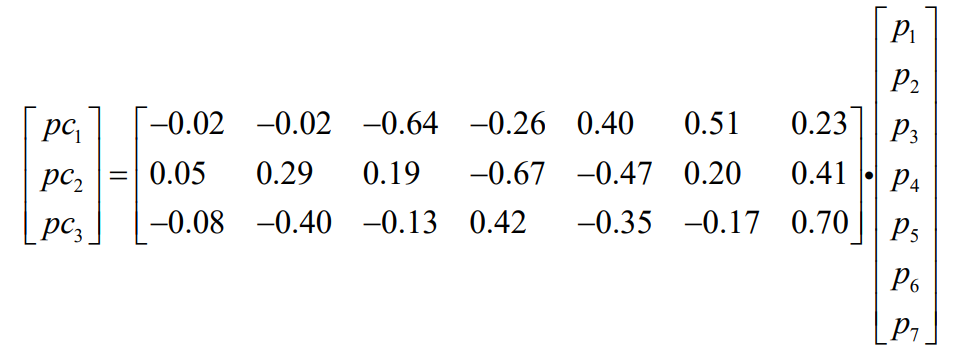
\includegraphics[width=0.7\linewidth]{pic/主成分.png}
    \label{matrix}
\end{figure}

Where $pc_i$ represents the $i$ principal component. For a principal component, the greater the coefficient before $P_n$, the greater the influence of the tries on the principal component.

The histogram (Figure \ref{pca}) in the left shows the percentage of explained variance for each component. The largest one reached a level of 70\%. The line chart in the right shows the accumulation of percentage of explained variance, through which we can see that 3 components contribute to about 98\% of explained variance. Therefore, the first three components we choose could fully represent the original variables.

\begin{figure}[hbt!]
    \centering
    \includegraphics[width=\linewidth]{pic/pca.png}
    \caption{Variance explained of principal component analysis}
    \label{pca}
\end{figure}

\subsubsection{Number of Cluster Points}

we used the elbow method and the silhouette coefficient to determine the value of $k$ as shown in Figure \ref{cluster points}.

\begin{figure}[hbt!]
    \centering
    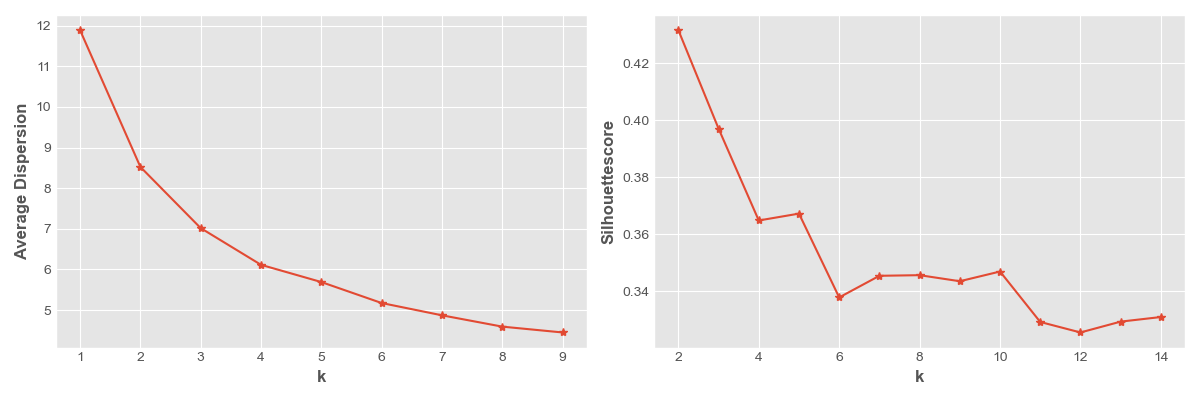
\includegraphics[width=\linewidth]{pic/聚类评价系数.png}
    \caption{The selection of cluster points numbe}
    \label{cluster points}
\end{figure}

In the elbow method, the decline slope of SSE decreases sharply at $k = 2 $ or 3. In the silhouette coefficient, the average silhouette coefficient is the largest when $k = 2$, followed by $k = 3$. Thus, the appropriate clustering number $k$ is 2 or 3. If $k = 2$, the difficulty can only be divided into two categories, which cannot fully explain the difficulty of the words. Therefore, we choose the clustering number $k = 3$. The difficulty of words is divided into three categories: difficult, medium and easy, and the k-means clustering analysis is carried out on them.

\subsubsection{K-means Clustering Algorithm}

Take $pc_1$ ,$pc_2$ and $pc_3$ as the x-y-z axis, and represent the data in the data set in the coordinate system, which can be roughly clustered into three categories as shown in the Figure \ref{The data set in the coordinate system}.

\begin{figure}[!htbp]
    \centering
    \subfigure[The data set in the coordinate system]{
        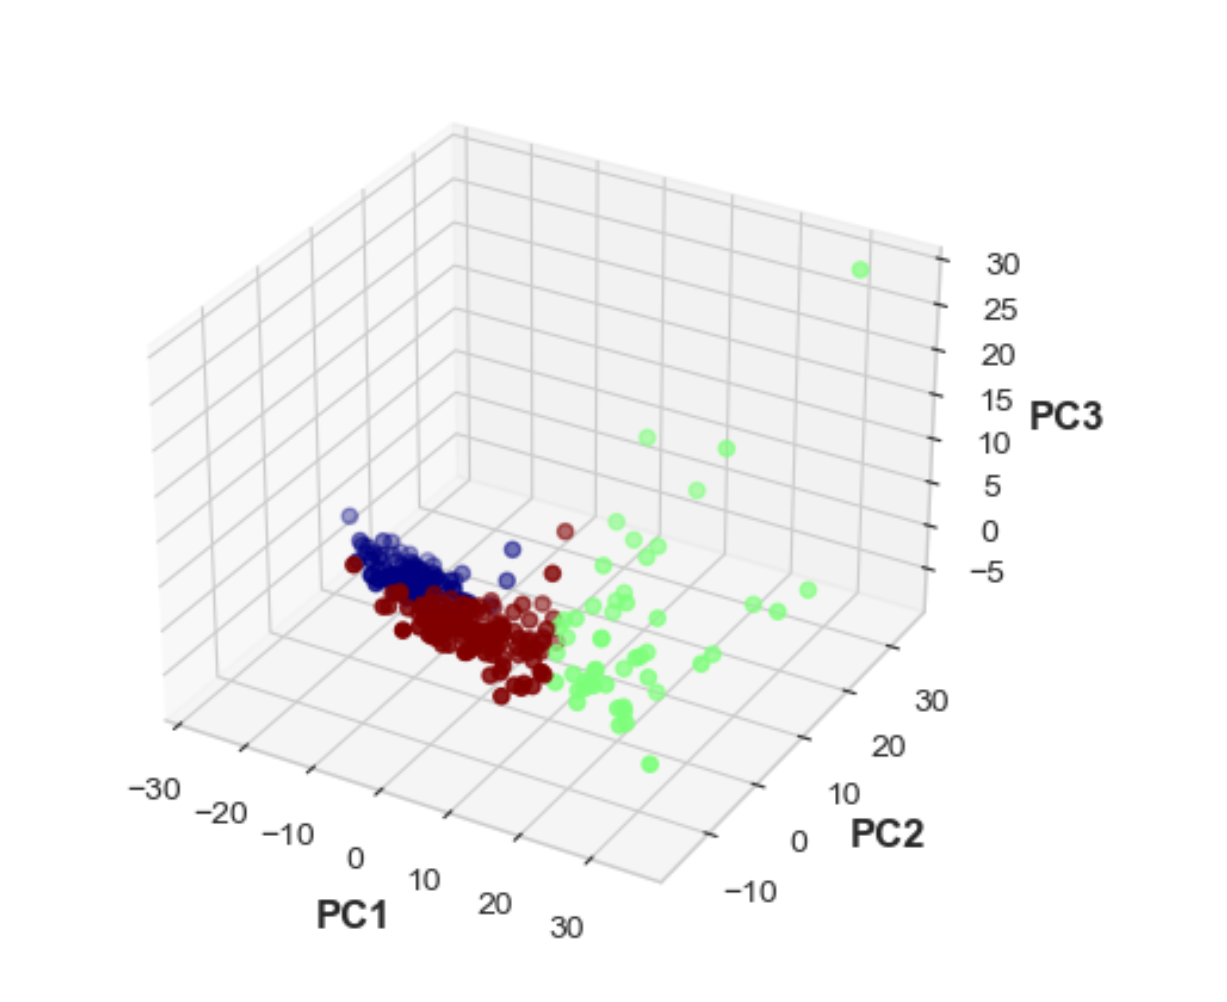
\includegraphics[width=0.49\linewidth]{pic/kmeans.png}
        \label{The data set in the coordinate system}
    }
    \hfill
    \subfigure[Cluster0: easy category]{
        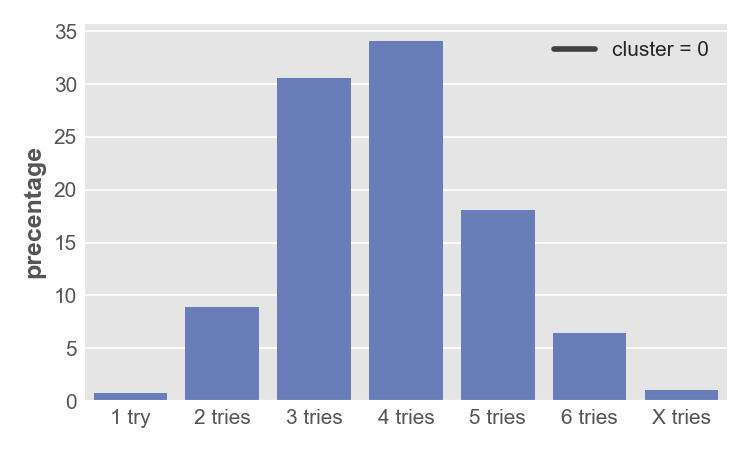
\includegraphics[width=0.49\linewidth]{pic/cluster0.png}
        \label{Cluster0: easy category}
    }
    \label{combine4}
\end{figure}

Detailed classification was carried out according to the above algorithm. After classification, average $P_n$ distribution in each category was taken, as shown in the figure. The average $P_n$ trend is obtained. According to the above, the more tries and the more difficult the words are, and the three categories cluster0 are easy, cluster2 is medium and cluster1 is difficult.

\begin{figure}[!htbp]
    \centering
    \subfigure[Cluster2: medium category]{
        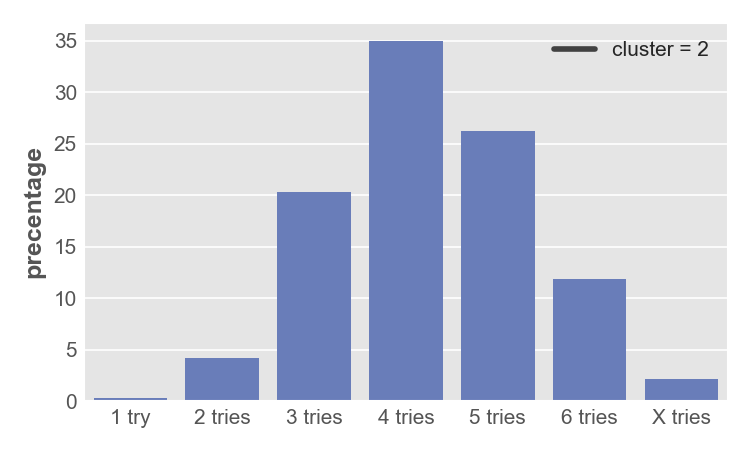
\includegraphics[width=0.49\linewidth]{pic/cluster2.png}
        \label{Cluster2: medium category}
    }
    \hfill
    \subfigure[Cluster1: difficult category]{
        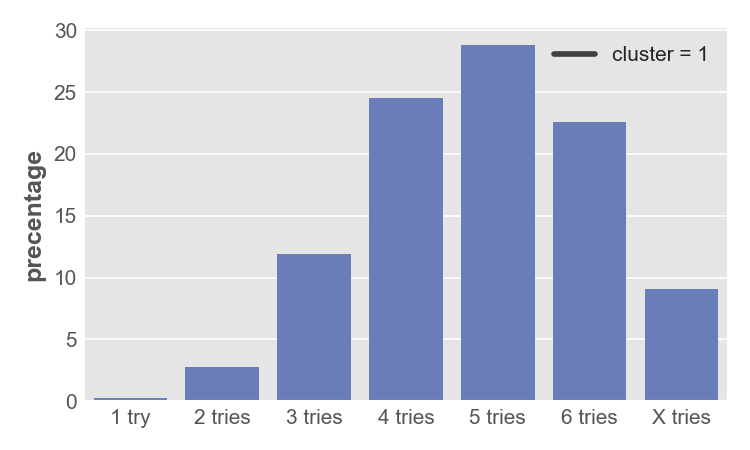
\includegraphics[width=0.49\linewidth]{pic/cluster1.png}
        \label{Cluster1: difficult category}
    }
    \label{combine5}
\end{figure}

\subsubsection{Words attributes of classifications}

To identify the relationship between attributes of and classifications, we refer to the first question, classify the qualitative data ‘part of speech’ as 0,1,2 according to the table 2, and take the average value of the word’s attributes in each classification, and radar maps are made for each category of difficult and easy, overlapped to observe the significant attributes in each category. outlining the attributes linked to each classification.

According to radar figure 1, date and word arrangement are not significant features. In radar figure 2, tags here refer to parts of speech, and parts of speech and number of vowels are not significant features. Clearly, the high frequency of letter and words usage is a significant attribute of the easy category, and the high number of repeated letters and combined letters is a significant attribute of the hard category.

\begin{figure}[!htbp]
    \centering
    \subfigure[]{
        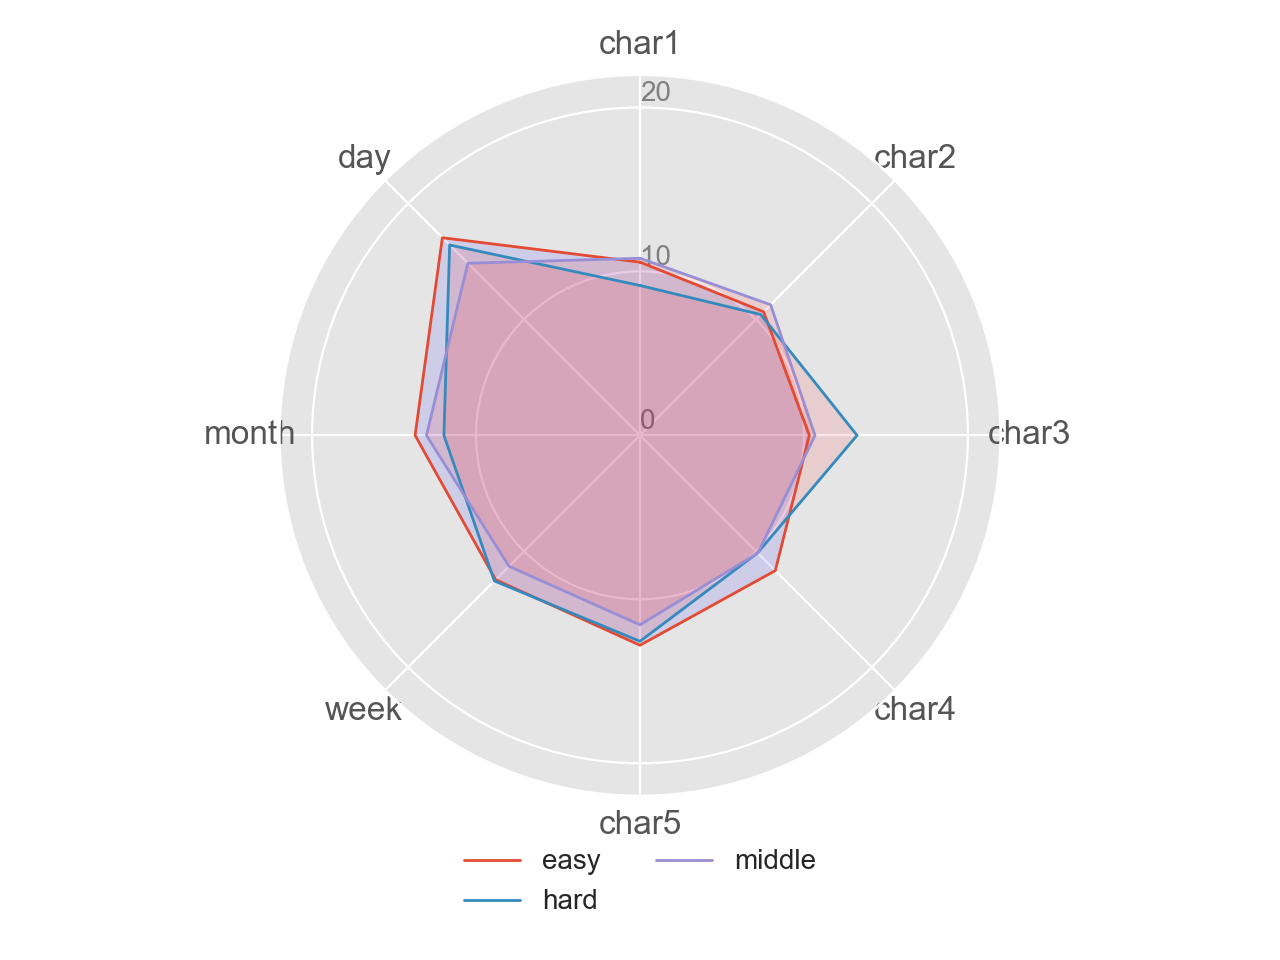
\includegraphics[width=0.49\linewidth]{pic/radius1.png}
        \label{Radar 1}
    }
    \hfill
    \subfigure[]{
        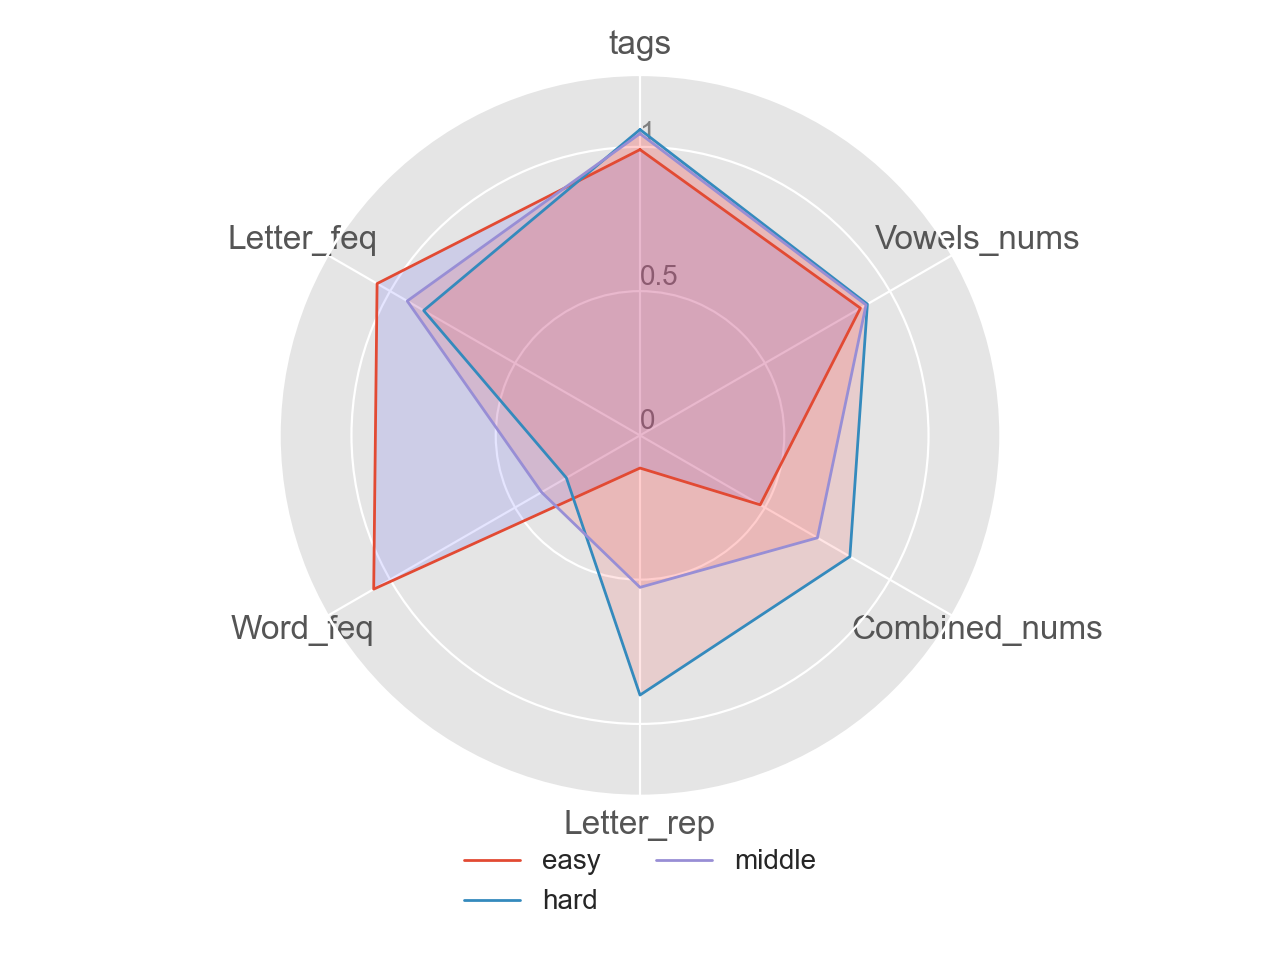
\includegraphics[width=0.49\linewidth]{pic/radius2.png}
        \label{Radar 2}
    }
    \caption{Radar maps of different attributes}
    \label{combine6}
\end{figure}

\subsubsection{Difficulty of Eerie}

According to the correlation percentage of eerie obtained in Model II, it is closest to the medium classification. Eerie has a low word usage frequency of 2272, a three-letter repetition, and a combined letters “er” which makes it difficult. But "E" is the most frequently used word, and the high frequency of the letters makes it easier to use more often. Therefore, it makes sense that it's medium difficulty.

\subsubsection{Accuracy}

The training set kmeans clustering has three central point data. The answer word in the question 2 is taken as the machine learning test set, and the principal component is calculated based on its real tries distribution. 

The classification represented by the nearest central point is taken as the correct classification of the test set words. GBDT Prediction Model was used to predict the distribution of tries of the test set and calculate the principal component. The classification represented by the nearest kmeans clustering center point of the training set was taken as the prediction classification of the words in the test set, and the prediction classification and correct classification were compared. Calculate the percentage of the same classification as the accuracy of the Word Difficulty Clustering Model. Using the classification report function in python, the classification report obtained by inputting the test set real data (y true) and predicted data (y pred) after the classification task is performed is often used to observe the quality of the model. f1-score and accuracy were used for evaluation.

\begin{table}[hbt!]
    \begin{threeparttable}
    \caption{Model accuracy judgement}
    \label{accuracy}
    \begin{tabular}{lllll}
    \toprule
    \headrow Class & Precision  & Recall & F1-score & Support\\ 
    \midrule
    easy & 0.76 & 0.83 & 0.79 & 30 \\ 
    \midrule
    medium & 0.82 & 0.73 & 0.77 & 11 \\ 
    \midrule
    hard & 0.90 & 0.85 & 0.87 & 31 \\ 
    \midrule
    accuracy &  &  & 0.79 & 72 \\ 
    \bottomrule 
    \end{tabular}
    \end{threeparttable}
\end{table}

The amount of test set is about 20 percent of the original data. The precision represents the proportion of samples correctly classified as positive examples in the proportion of samples classified as positive examples. The recall rate is the proportion of samples correctly classified positive cases to the proportion of positive cases in the original data. F1-score is the harmonic average as formula below. Where $P$ means precision and R means recall. Support refers to the number of original real data belonging to this class. Accuracy refers to the rate of correct classification. 

$$\frac{1}{F_1} = \frac{1}{2}*(\frac{1}{P}+\frac{1}{R})$$

As shown in the table \ref{accuracy}, the accuracy of the model is relatively high, and the values are all around 0.8. 

\section{Feature Correlation Exploration}

Correlation analysis is carried out on the seven try features, and a scatter plot is made in pairs. The coordinate axis of the figure 17 is from 1 try to 7 tries from top to bottom, and from left to right. We can generalize interesting properties from the population correlation scatter plot, and there is a strong correlation between certain trial features. Taking 3tries and 5 tries as an example, it is obvious that there is a negative correlation between the two. The bigger 5 tries is, the smaller 3 tries is, and there is a strong negative linear correlation. It can be interpreted that the bigger 5 tries is, the less common a word is, so the lower the probability of getting 3tries. The fewer times it appears; Similarly, 3 tries has a strong negative linear correlation with 6 tries and 7 tries. On the contrary, it can be observed that there is a strong positive correlation between 3 tries and 2 tries. The higher the value of 3 tries, the higher the value of 2tries, which can also be explained by the difficulty of the word. Therefore, to some extent, we corroborate the difficulty classification method in the model III. It is worth noting that according to the dispersion degree of the scatter chart, 4 tries does not seem to have a strong correlation with other tries, which indicates that it is difficult for the feature of 4 tries to have a strong correlation with other features. Therefore, to some extent, this also explains the reason why the prediction accuracy of 4 tries in the model II is low.

\begin{figure}[hbt!]
    \centering
    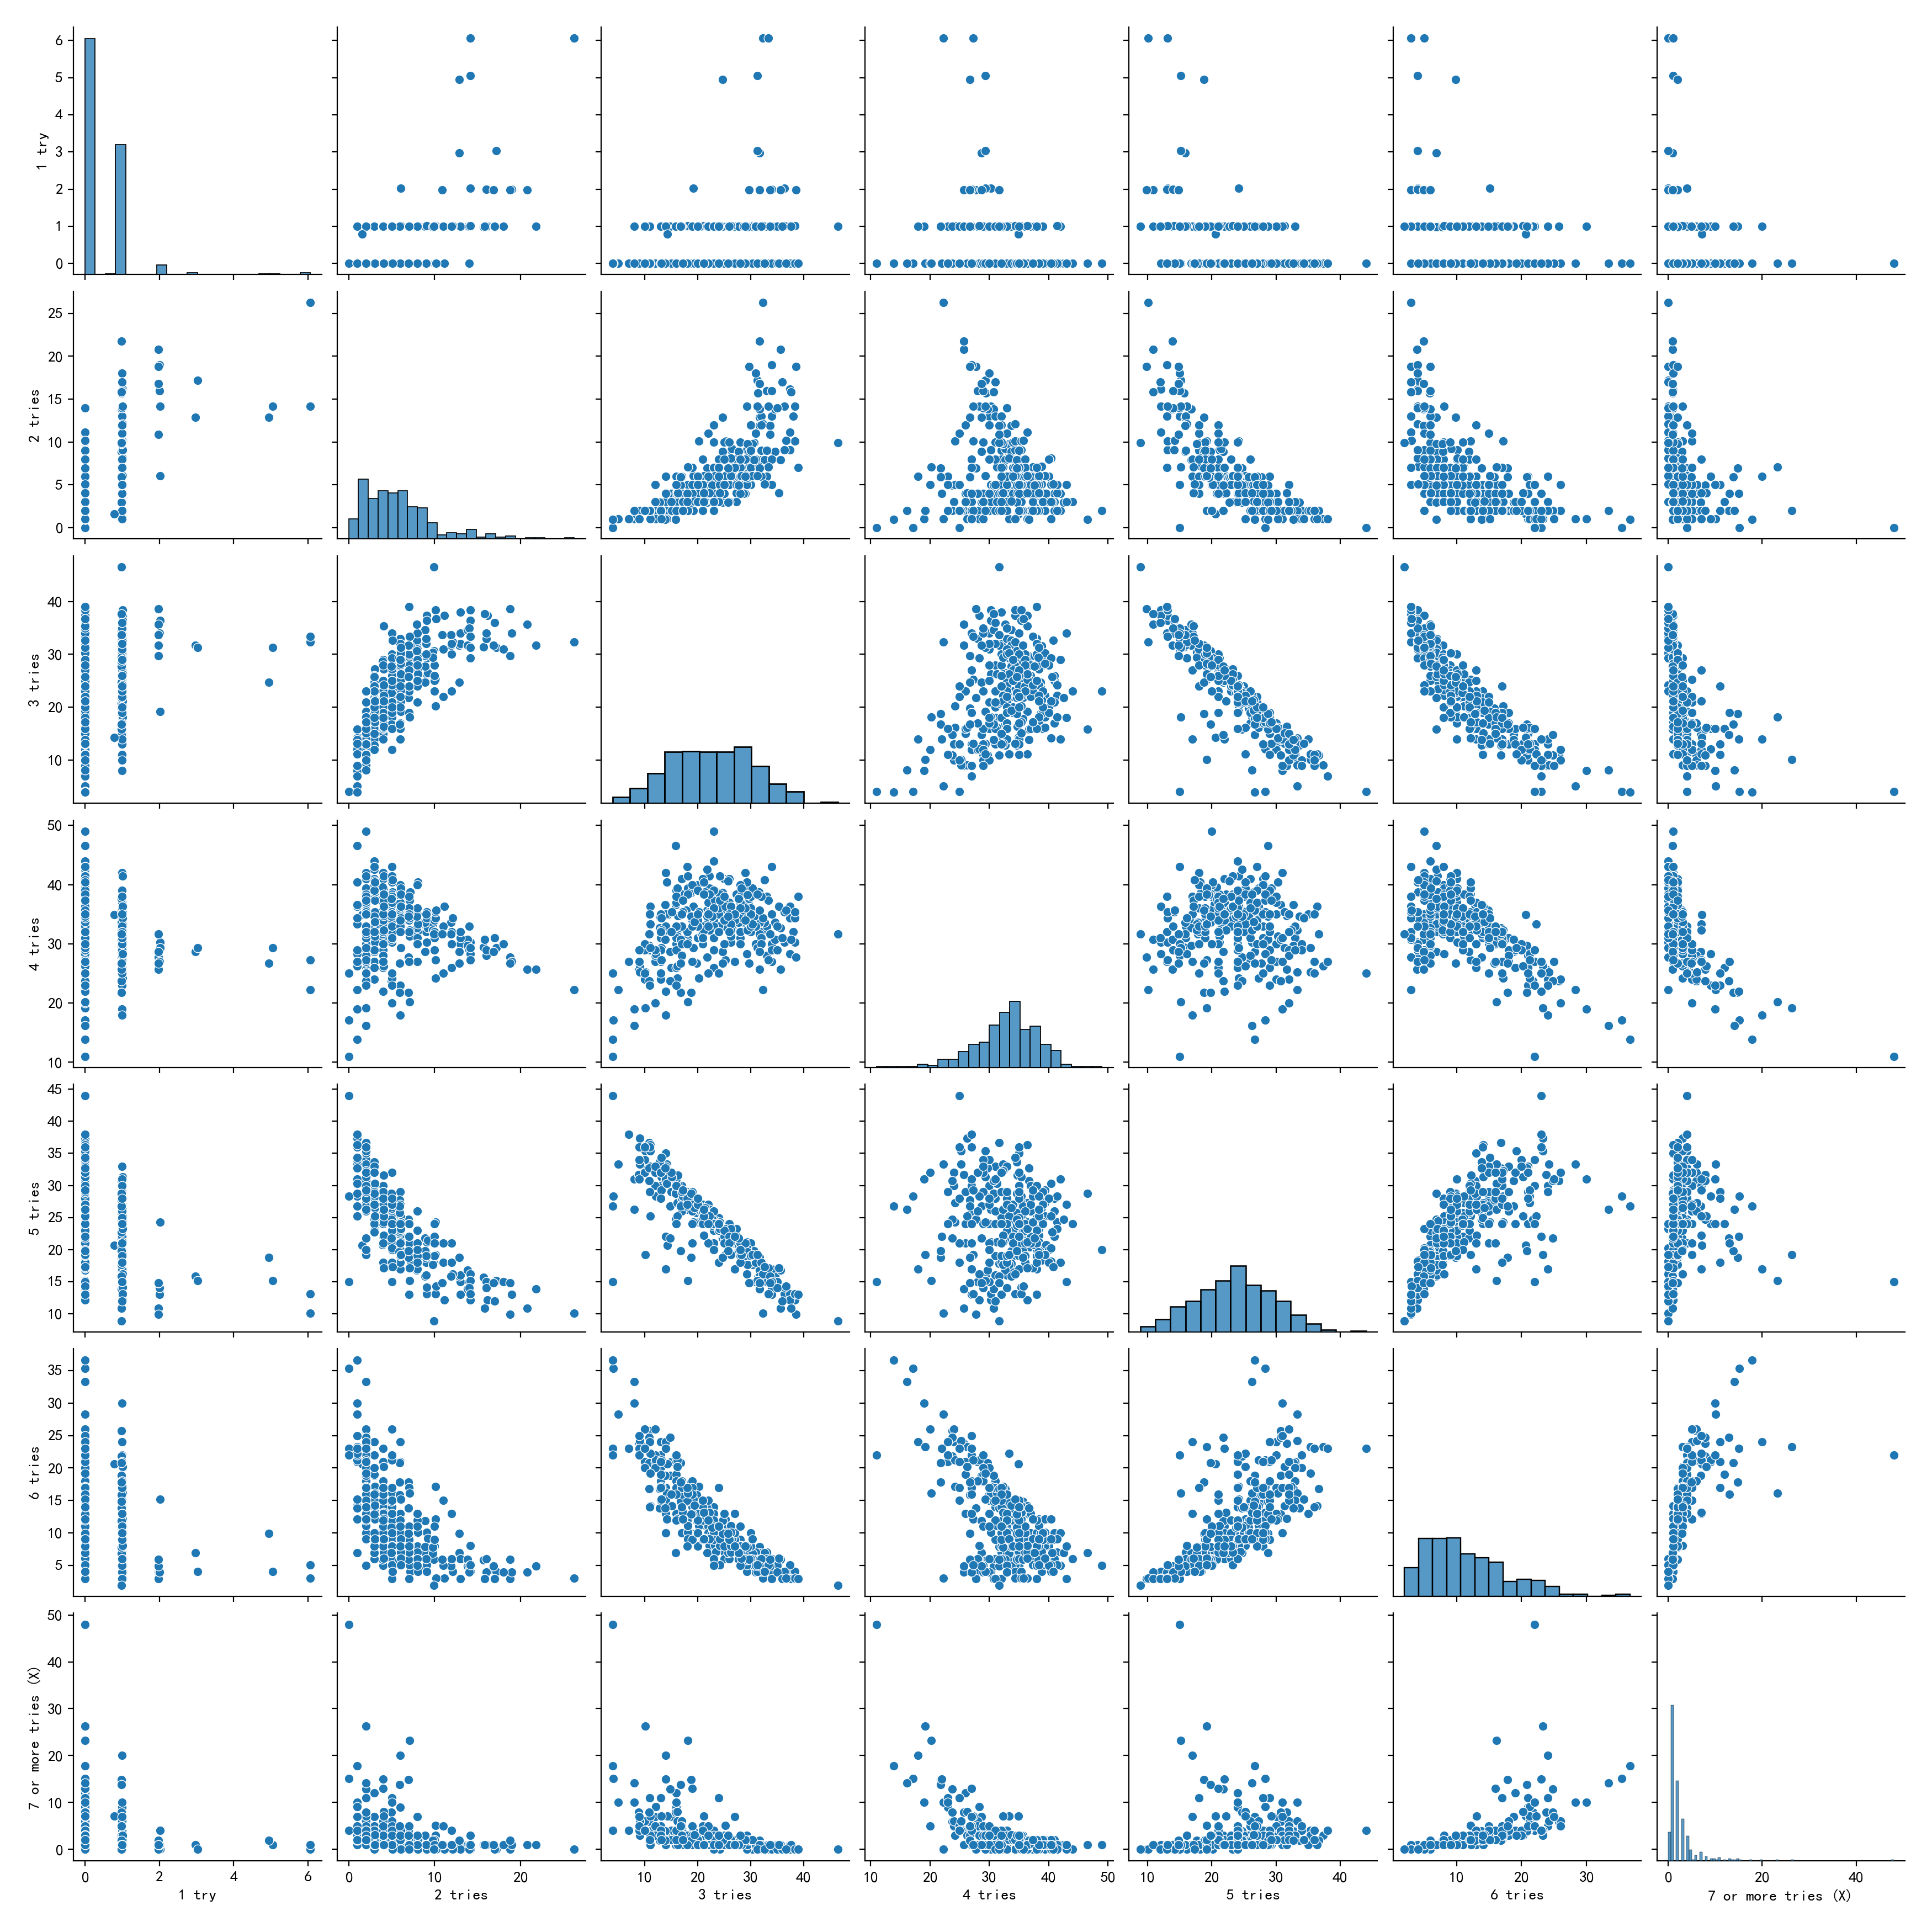
\includegraphics[width=\linewidth]{pic/tries相关性图.png}
    \caption{Scatter plot of 1 try to 7 tries}
    \label{scatter}
\end{figure}

Therefore, to some extent, we corroborate the difficulty classification method in the model III. It is worth noting that according to the dispersion degree of the scatter chart, 4 tries does not seem to have a strong correlation with other tries, which indicates that it is difficult for the feature of 4 tries to have a strong correlation with other features. Therefore, to some extent, this also explains the reason why the prediction accuracy of 4 tries in the model II is low.

The correlation between the number of reported results and the number in hard mode (Figure \ref{two relation}) was analyzed and the scatter diagram was made as figure 18. It can be seen from observation that the two have a strong correlation. The more the number of reported results, However, we found that there was a trend of two regression lines, which may be caused by two positive correlation mechanisms between the Number of reported results and the Number in hard mode, which is worth further study.

\begin{figure}[hbt!]
    \centering
    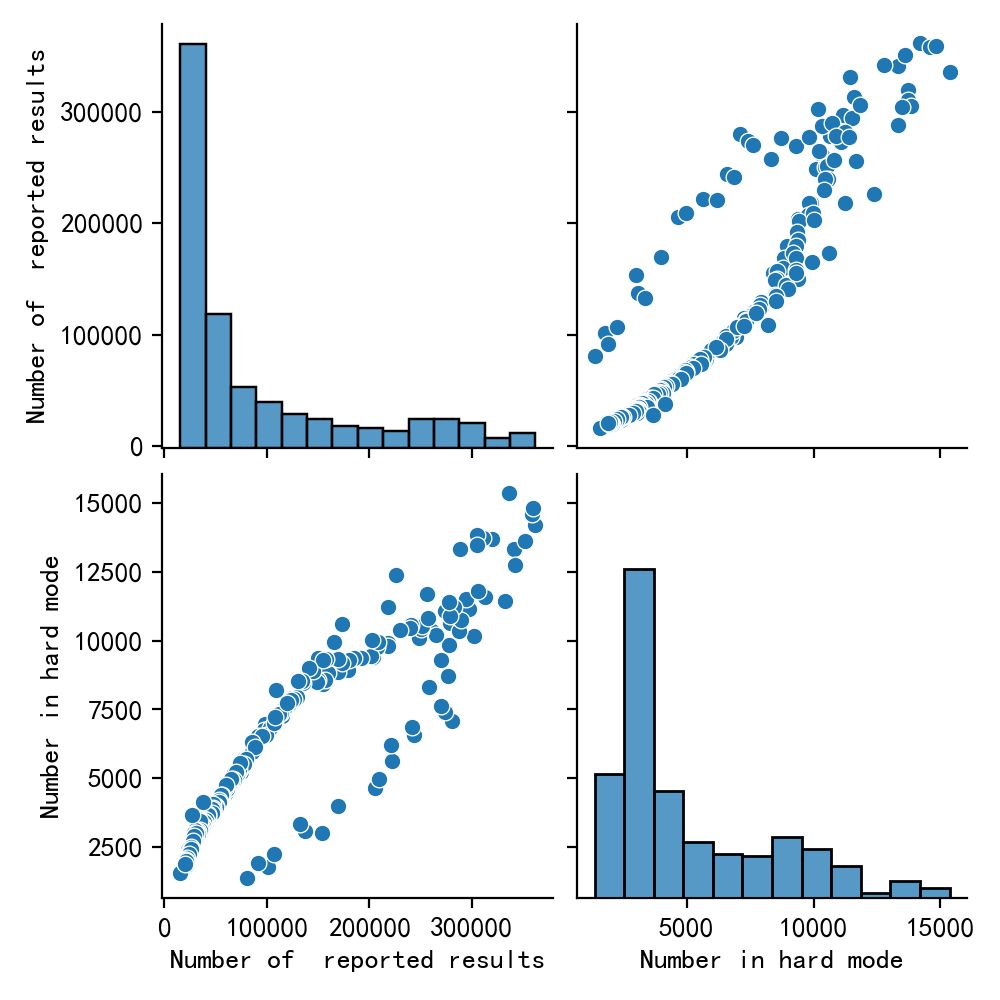
\includegraphics[width=0.5\linewidth]{pic/Numbers相关性图.png}
    \caption{The correlation between reported results and hard mode}
    \label{two relation}
\end{figure}

\section{Sensitivity Analysis}

In section 5.1, we get the differential relationship between the parameter $\alpha$, $\beta$, $\gamma_n$, $N'$ and the number of people participating in the report. Take the partial derivative of each of the four parameters. The partial derivative of the parameter with respect to $I_{418}'$ is shown in Figure \ref{Sen 1}. The partial derivative of the parameter with respect to $\Delta \overline{I}$ is shown in Figure \ref{Sen 2}. The partial derivatives of the four parameters of the model are calculated and their slopes are observed. The slope of parameter $\alpha$ is the highest, indicating that it had the greatest influence on the model. Since there is no infinite value, the model performs well in sensitivity analysis. 

\begin{figure}[!htbp]
    \centering
    \subfigure[The partial derivative of the parameter with respect to $I_{418}'$]{
        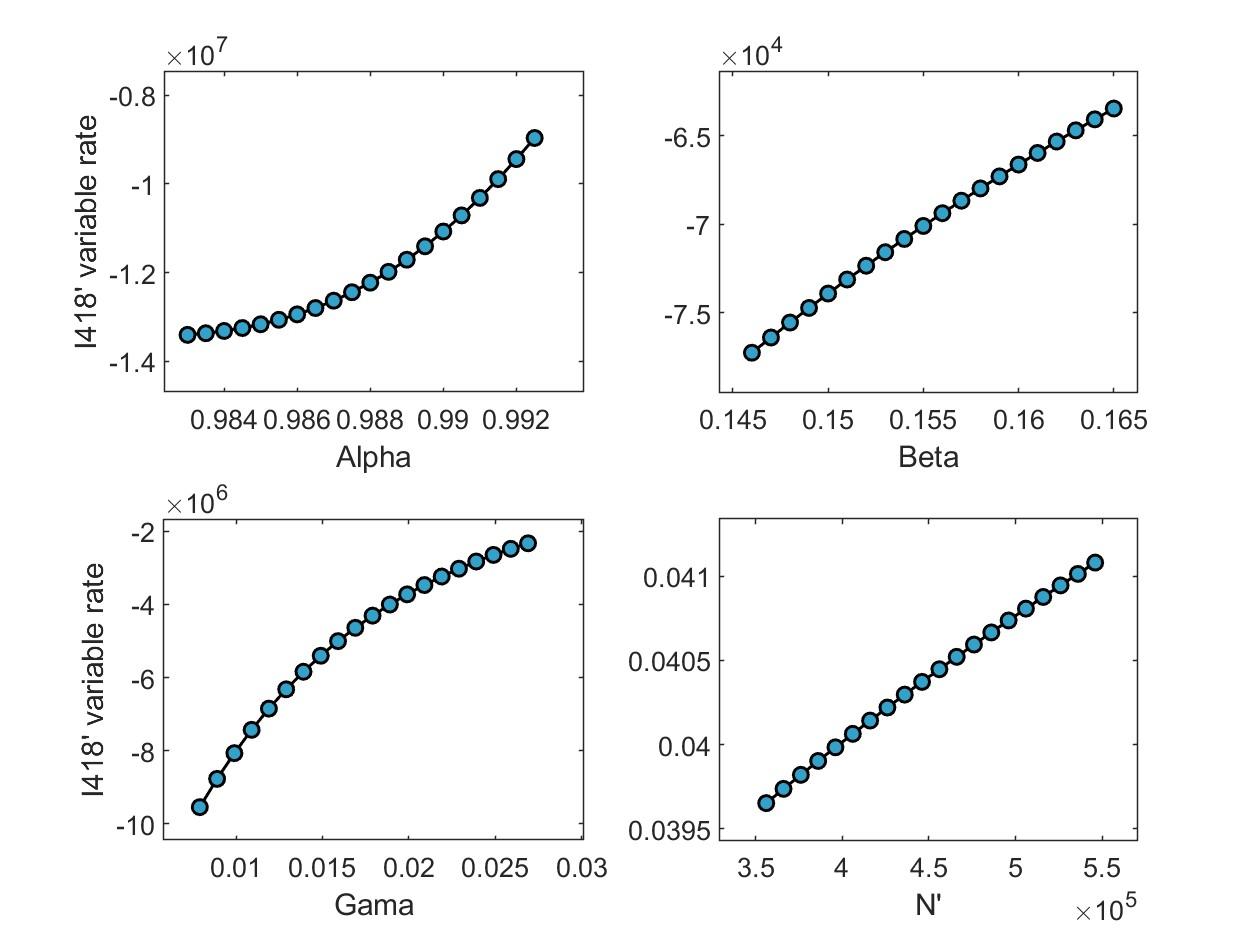
\includegraphics[width=0.49\linewidth]{pic/sen1.jpg}
        \label{Sen 1}
    }
    \hfill
    \subfigure[The partial derivative of the parameter with respect to $\Delta \overline{I}$ ]{
        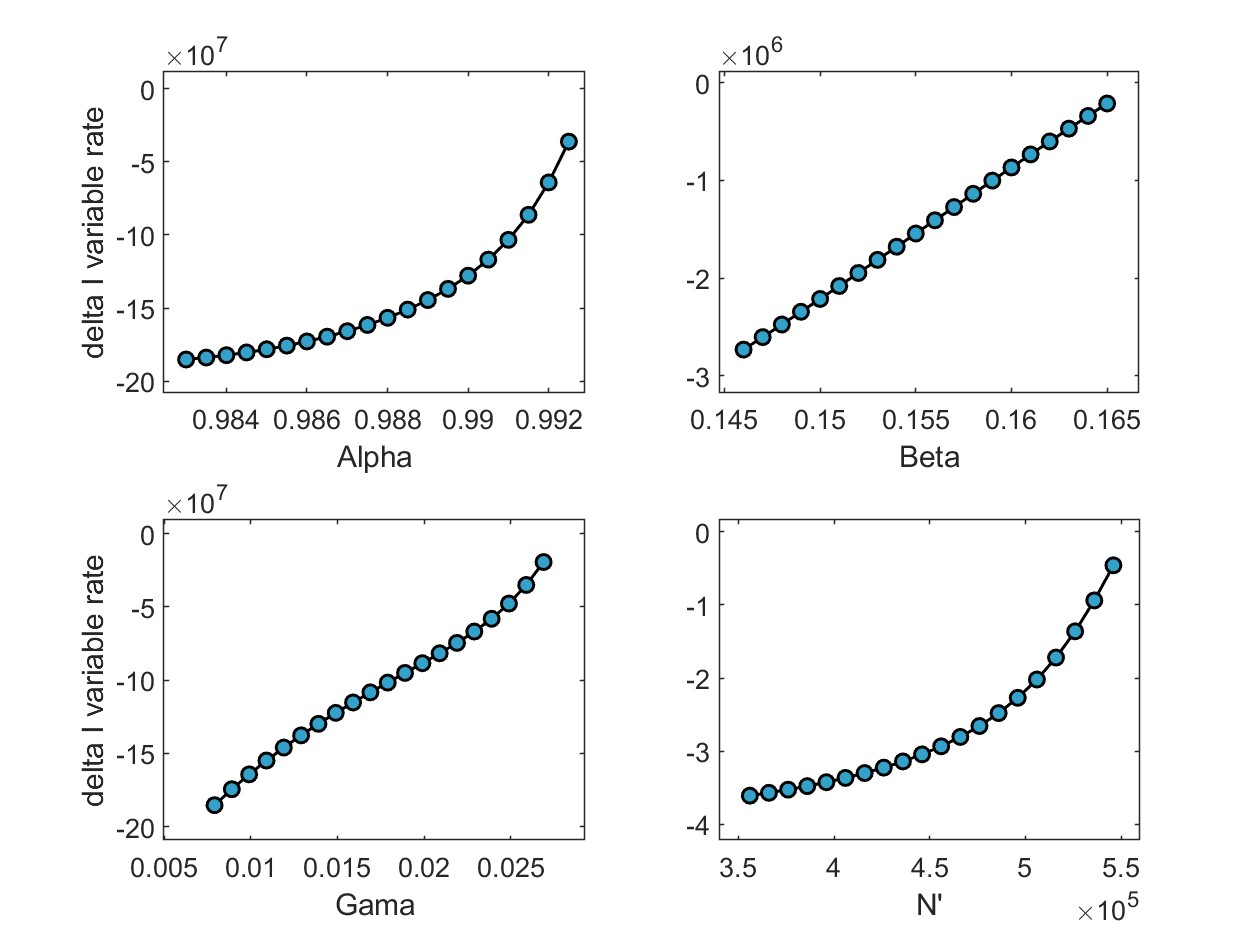
\includegraphics[width=0.49\linewidth]{pic/sen2.jpg}
        \label{Sen 2}
    }
    \label{combine7}
\end{figure}

\section{Conclusion}
\subsection{Strengths}
$\bullet$ The reported number prediction algorithm refers to the SIR epidemic disease model. From the principle, it can describe and explain the changes of the total number of reports well. After passing the sensitivity test, the prediction results obtained have certain mathematical support and are scientific and reasonable;

$\bullet$ The reported results distribution prediction model uses a mature GBDT machine learning algorithm, which can mine possible nonlinear relationships and has relatively high prediction accuracy;

$\bullet$ This paper establishes a set of objective and reasonable definition methods for difficulty classification, and combines the distribution prediction model to realize the conversion from word features to difficulty classification with high accuracy. 

\subsection{Possible Improvements}

$\bullet$ The report number prediction model does not have the ability to explain the fluctuation of data on a relatively short time scale. Combined with the report result distribution prediction model of Question 2 and the possible relationship between the result distribution and the sharing rate, the model can be modified to reflect the volatility to a certain extent;

$\bullet$ Predictions of the distribution of reported results can be more accurate if we have larger amounts of data.

\section{References}

[1] Anderson, B. J., Meyer, J. G. (2022). Finding the optimal human strategy for Wordle using maximum correct letter probabilities and reinforcement learning. 

https://doi.org/10.48550/ARXIV.2202.00557 

[2] Mata, A. S., Dourado, S. M. P. (2021). Mathematical modeling applied to epidemics: An overview. São Paulo Journal of Mathematical Sciences, 15(2), 1025–1044. https://doi.org/10.1007/s40863-021-00268-7 

[3] Friedman, J. H. (2001). Greedy function approximation: A gradient boosting machine. The Annals of Statistics, 29(5). https://doi.org/10.1214/aos/1013203451 

[4] Abdi, H. and Williams, L.J. (2010), Principal component analysis. WIREs Comp Stat, 2: 433-459. https://doi.org/10.1002/wics.101 

[5] Arthur, D., Vassilvitskii, S. (n.d.). k-means++: The Advantages of Careful Seeding.

\end{document}